\section{Characterization of MAPMTs}

\begin{figure*}[hbt] 
\centering 
  \subfloat[3 mm mask]{%
    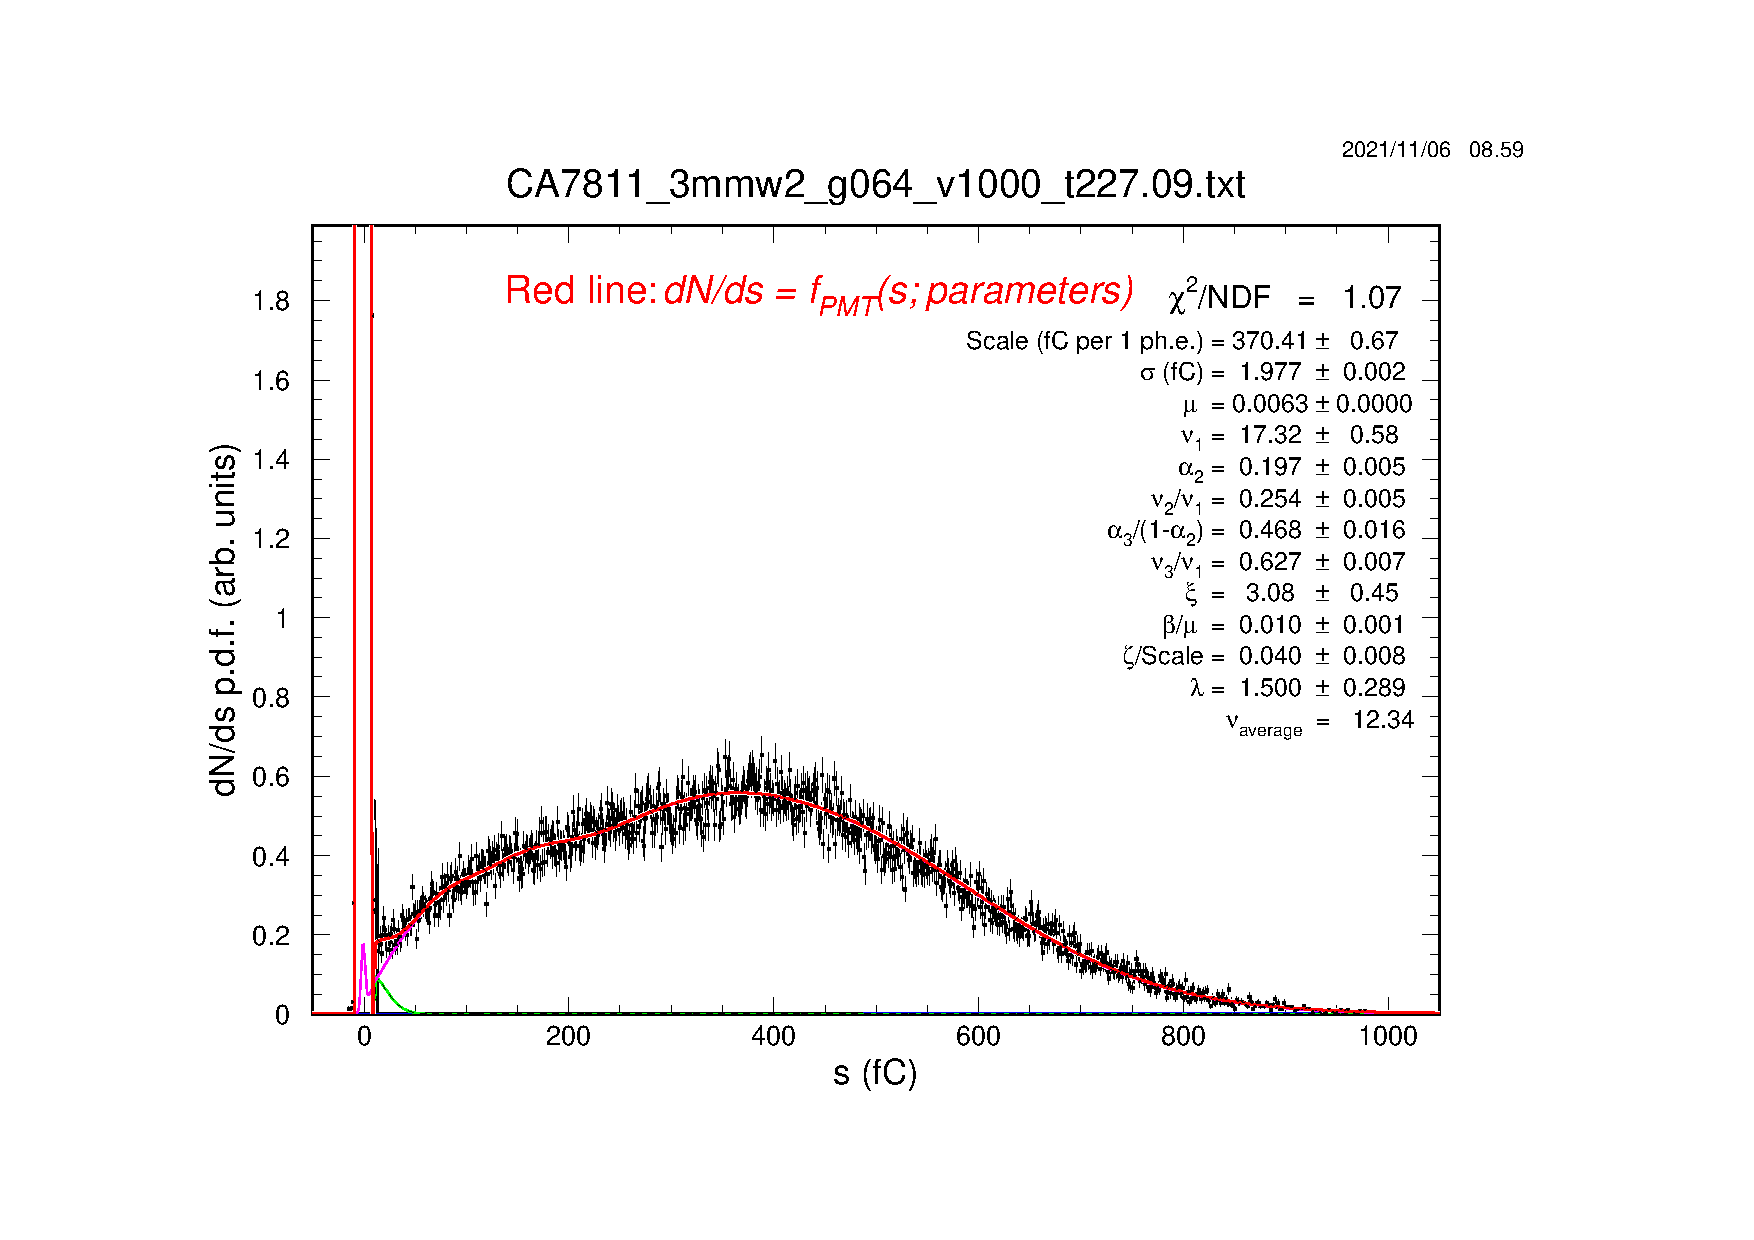
\includegraphics[clip=true,trim=100 75 140 100,width=.49\textwidth,height=.25\textwidth]
                    {figures/CA7811_a.pdf}}
  \subfloat[6 mm mask]{%
    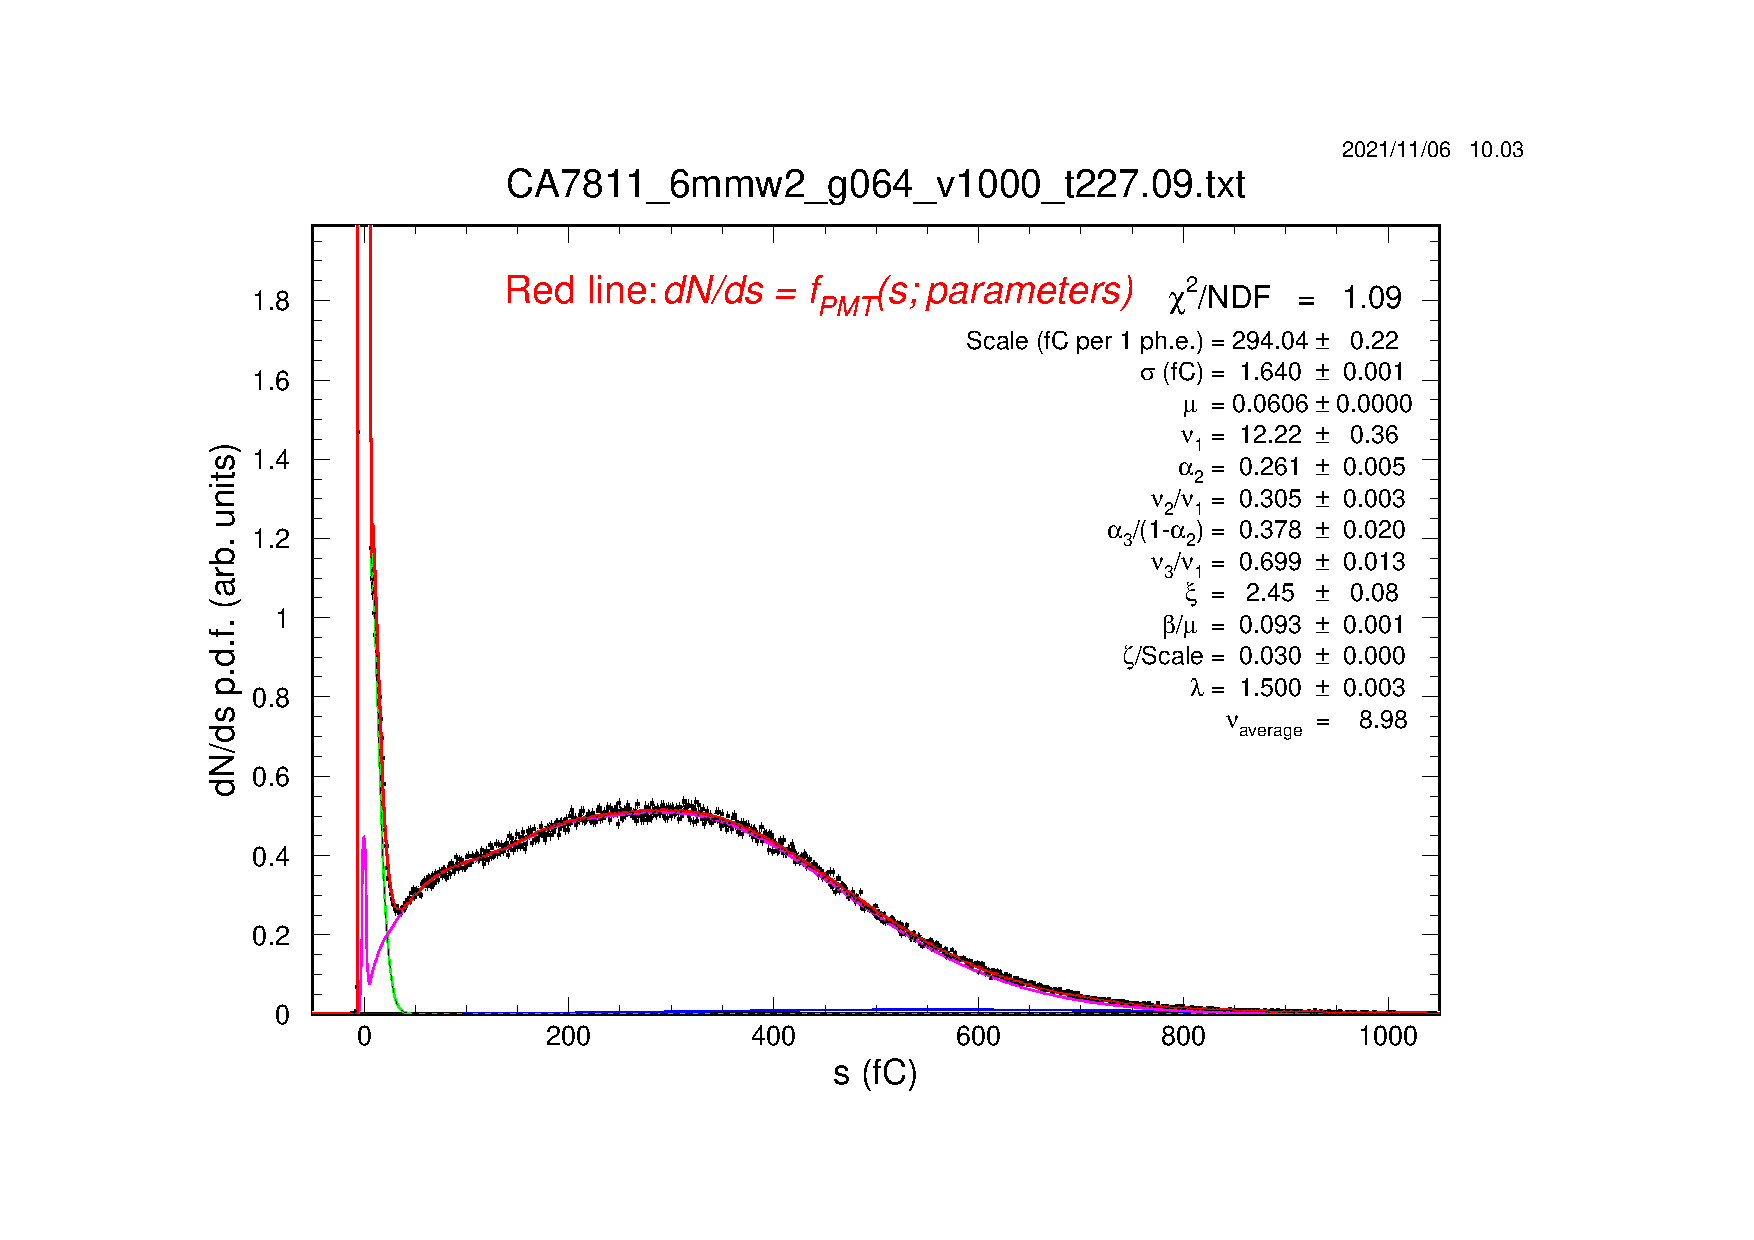
\includegraphics[clip=true,trim=100 75 140 100,width=.49\textwidth,height=.25\textwidth]
                    {figures/CA7811_b.pdf}} \\
  \subfloat[No mask, cross talk removed by software]{%
    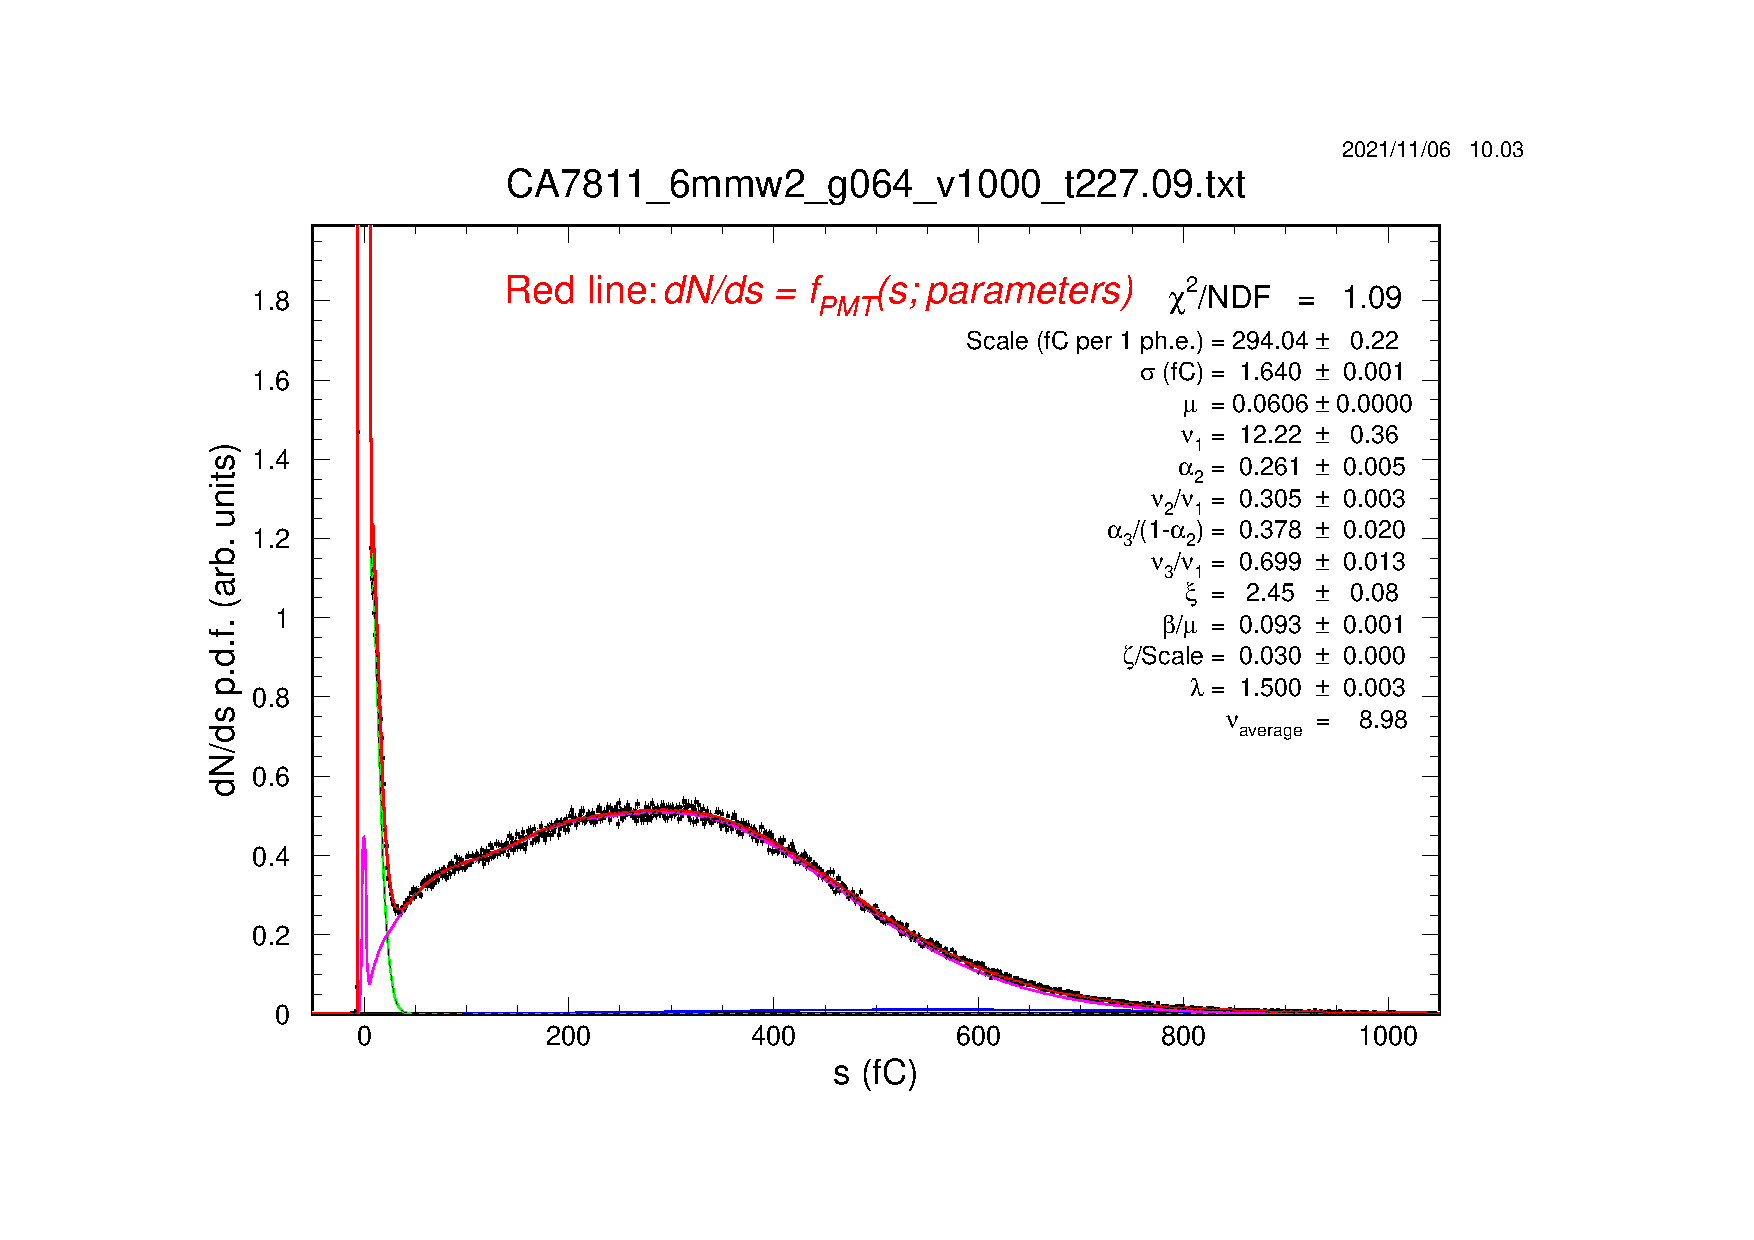
\includegraphics[clip=true,trim=100 75 140 100,width=.49\textwidth,height=.25\textwidth]
                    {figures/CA7811_c.pdf}}
  \subfloat[No mask, cross talk approximated by fit]{%
    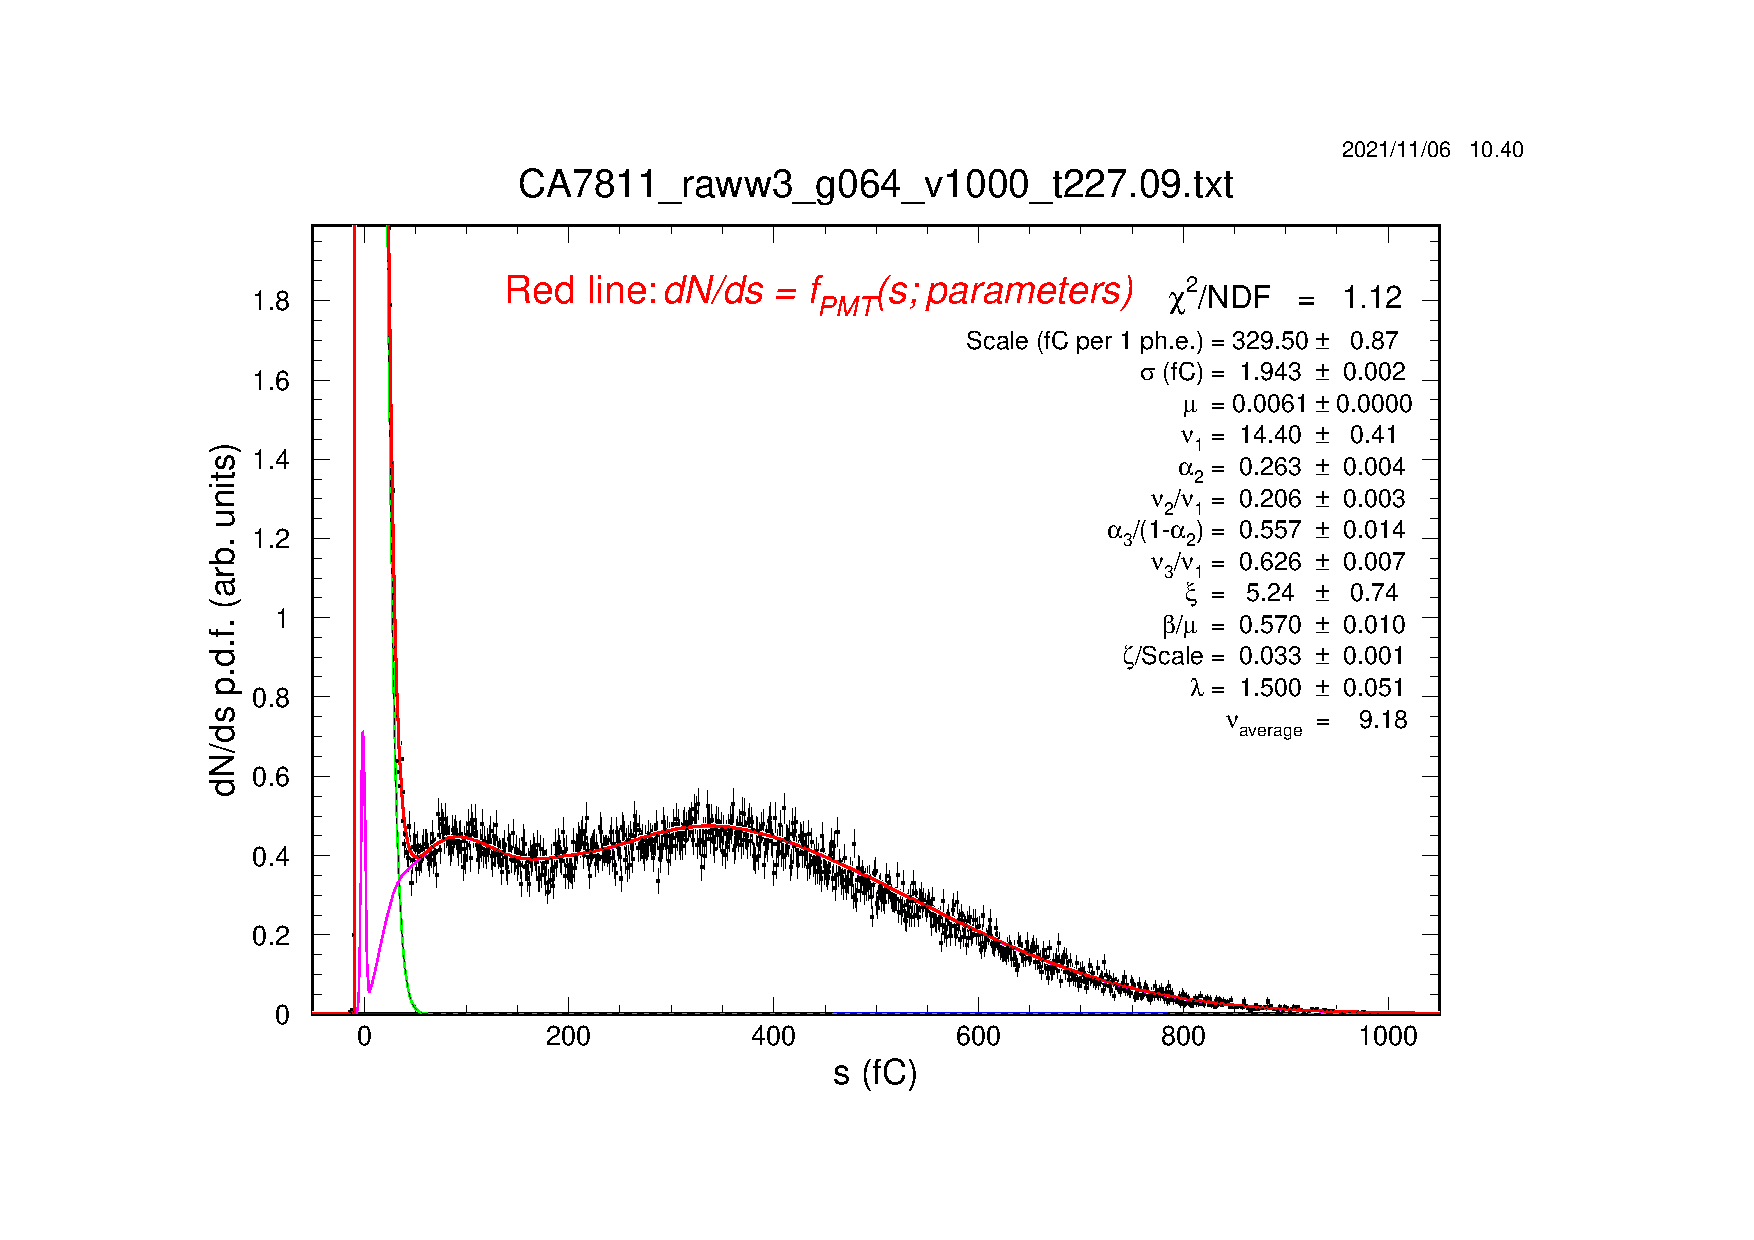
\includegraphics[clip=true,trim=100 75 140 100,width=.49\textwidth,height=.25\textwidth]
                    {figures/CA7811_d.pdf}}
  \caption{Signal amplitude probability distributions for PMT CA7811 (H8500), pixel 9, at HV = 1000 V. The signal amlitude $s$ is in units of fC, and the measured spectra are shown as black dots with statistical errors. Red lines correspond to the parameterized model charge distributions. Green and violet lines correspond to $m=0$ and $m=1$ functions as explained in Fig.~\ref{fig:Model}. Subplots: (a) 3~mm mask; (b) 6~mm mask; (c) run with full PMT face open with the crosstalk events removed by the correlation analysis; (d) run with full PMT face open, with the contribution to the spectrum from the crosstalk events approximated and parameterized by the analysis algorithm. The crosstalk effects in the open configuration are too wide, the fitting algorithm cannot distinguish between the crosstalk and the SPE distribution, and the evaluated SPE function in the (d) plot differs from the ``clean'' one in the (c) plot.
    }
\label{fig:CA7811}
\end{figure*}

\begin{figure*}[hbt] 
\centering 
  \subfloat[3 mm mask]{%
    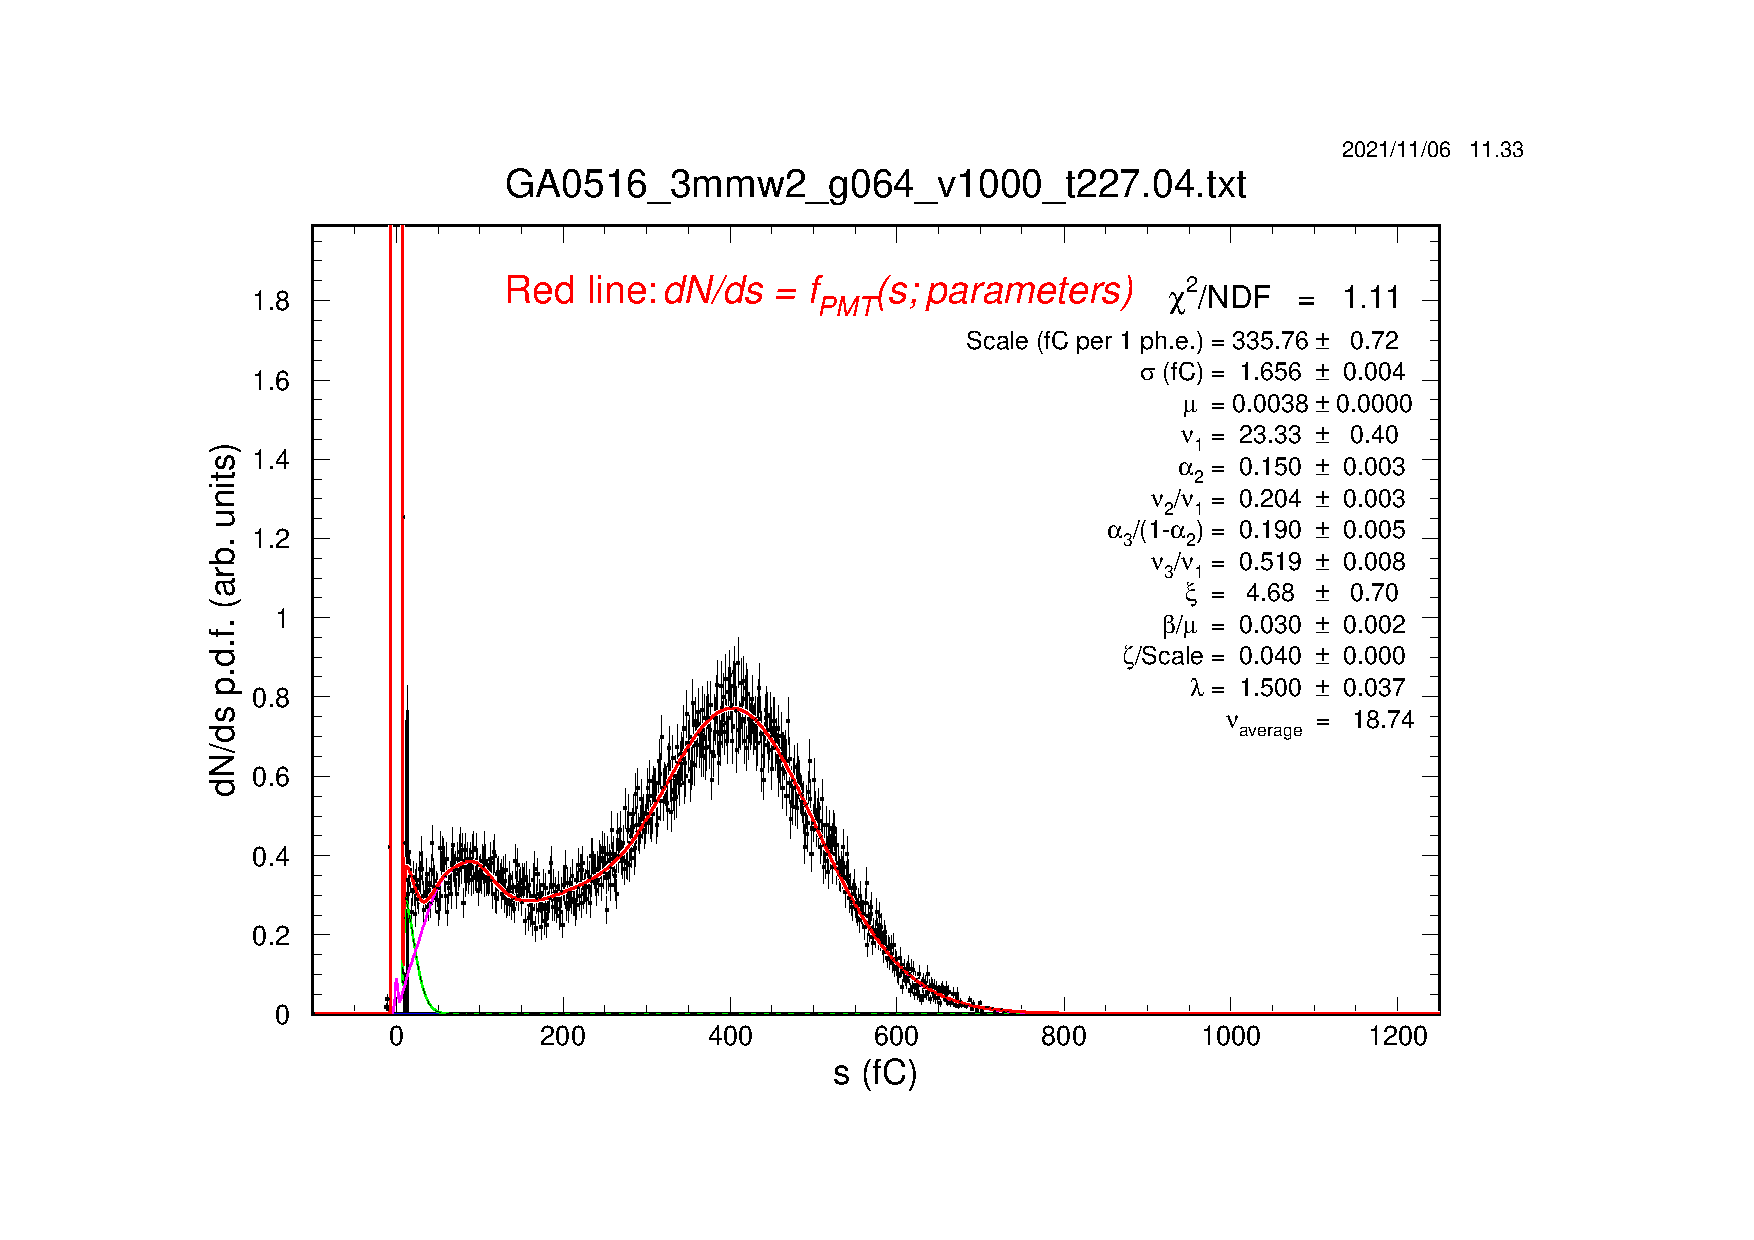
\includegraphics[clip=true,trim=100 75 140 100,width=.49\textwidth,height=.25\textwidth]
                    {figures/GA0516_1a.pdf}}
  \subfloat[6 mm mask]{%
    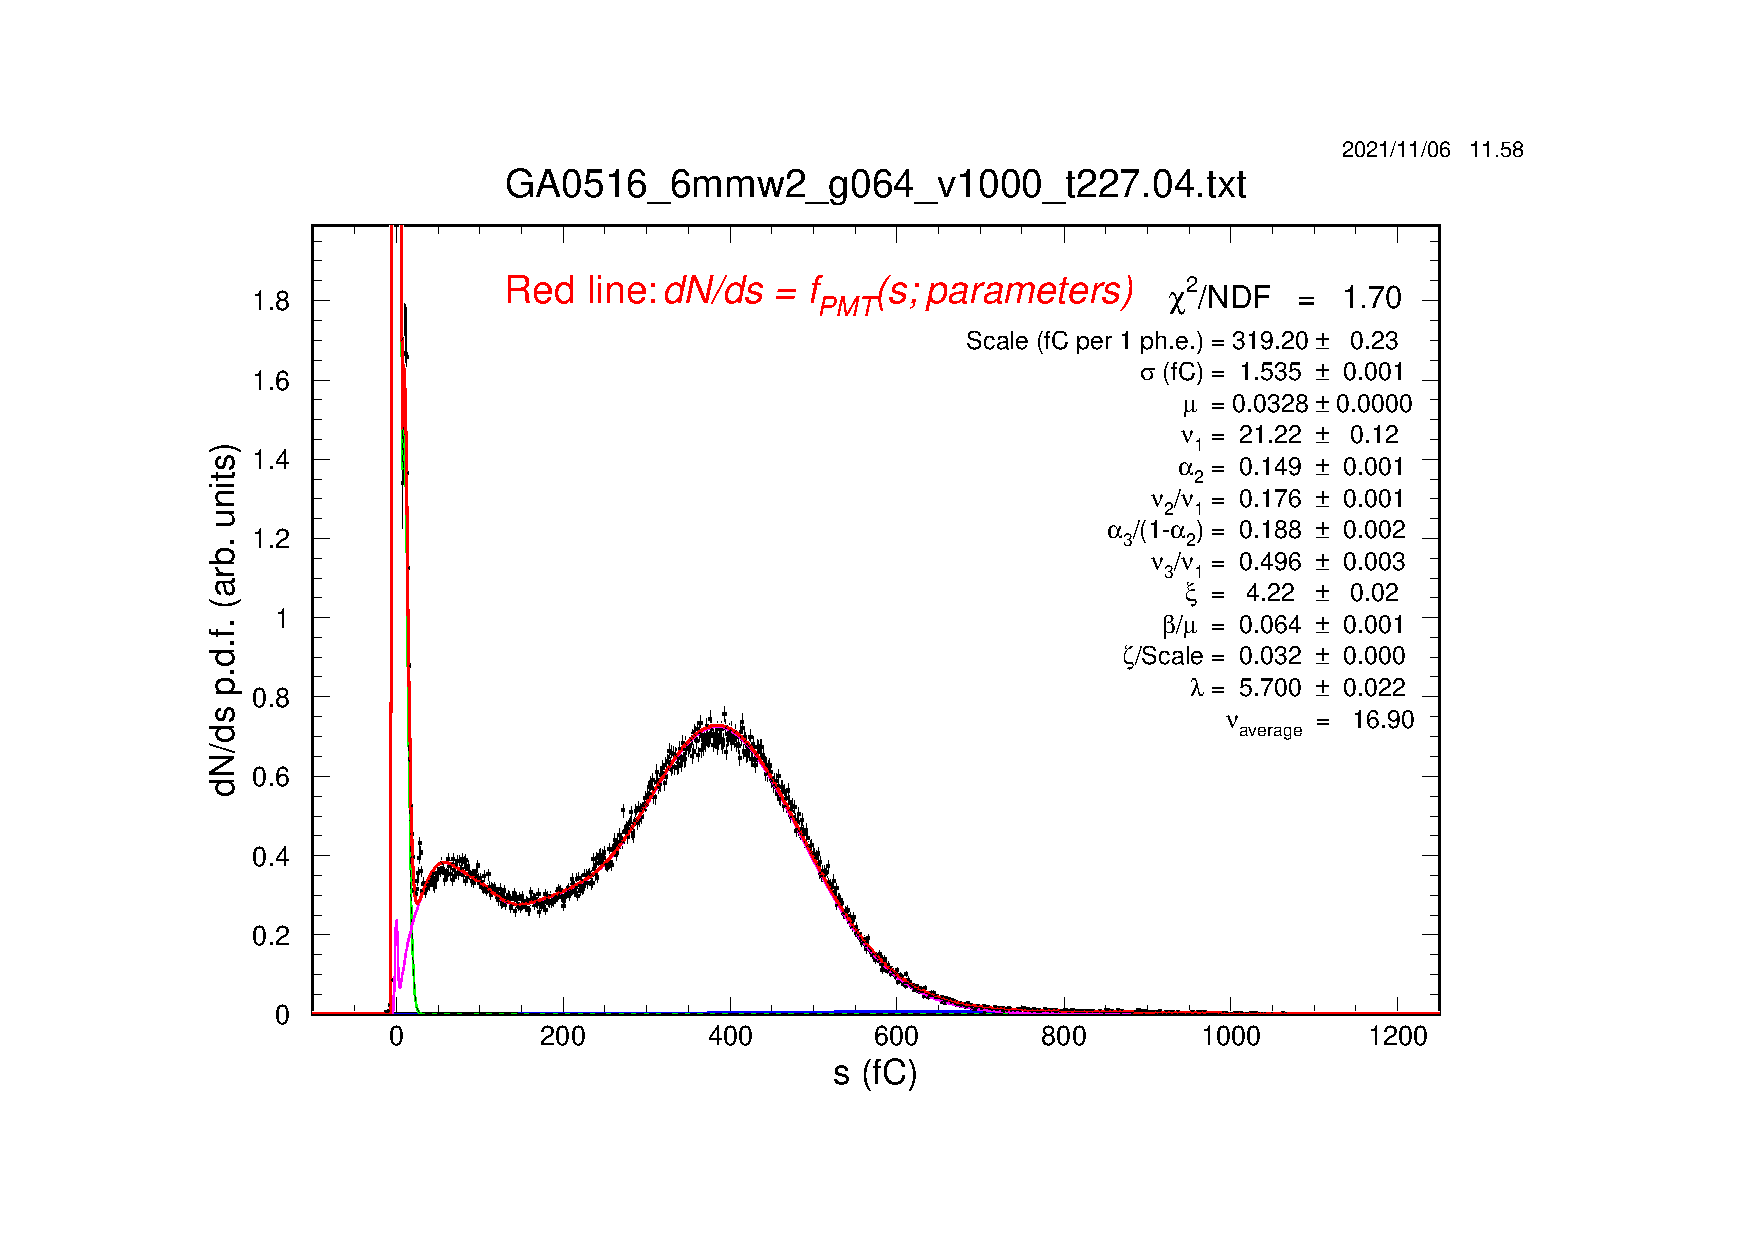
\includegraphics[clip=true,trim=100 75 140 100,width=.49\textwidth,height=.25\textwidth]
                    {figures/GA0516_1b.pdf}} \\
  \subfloat[No mask, cross talk removed by software]{%
    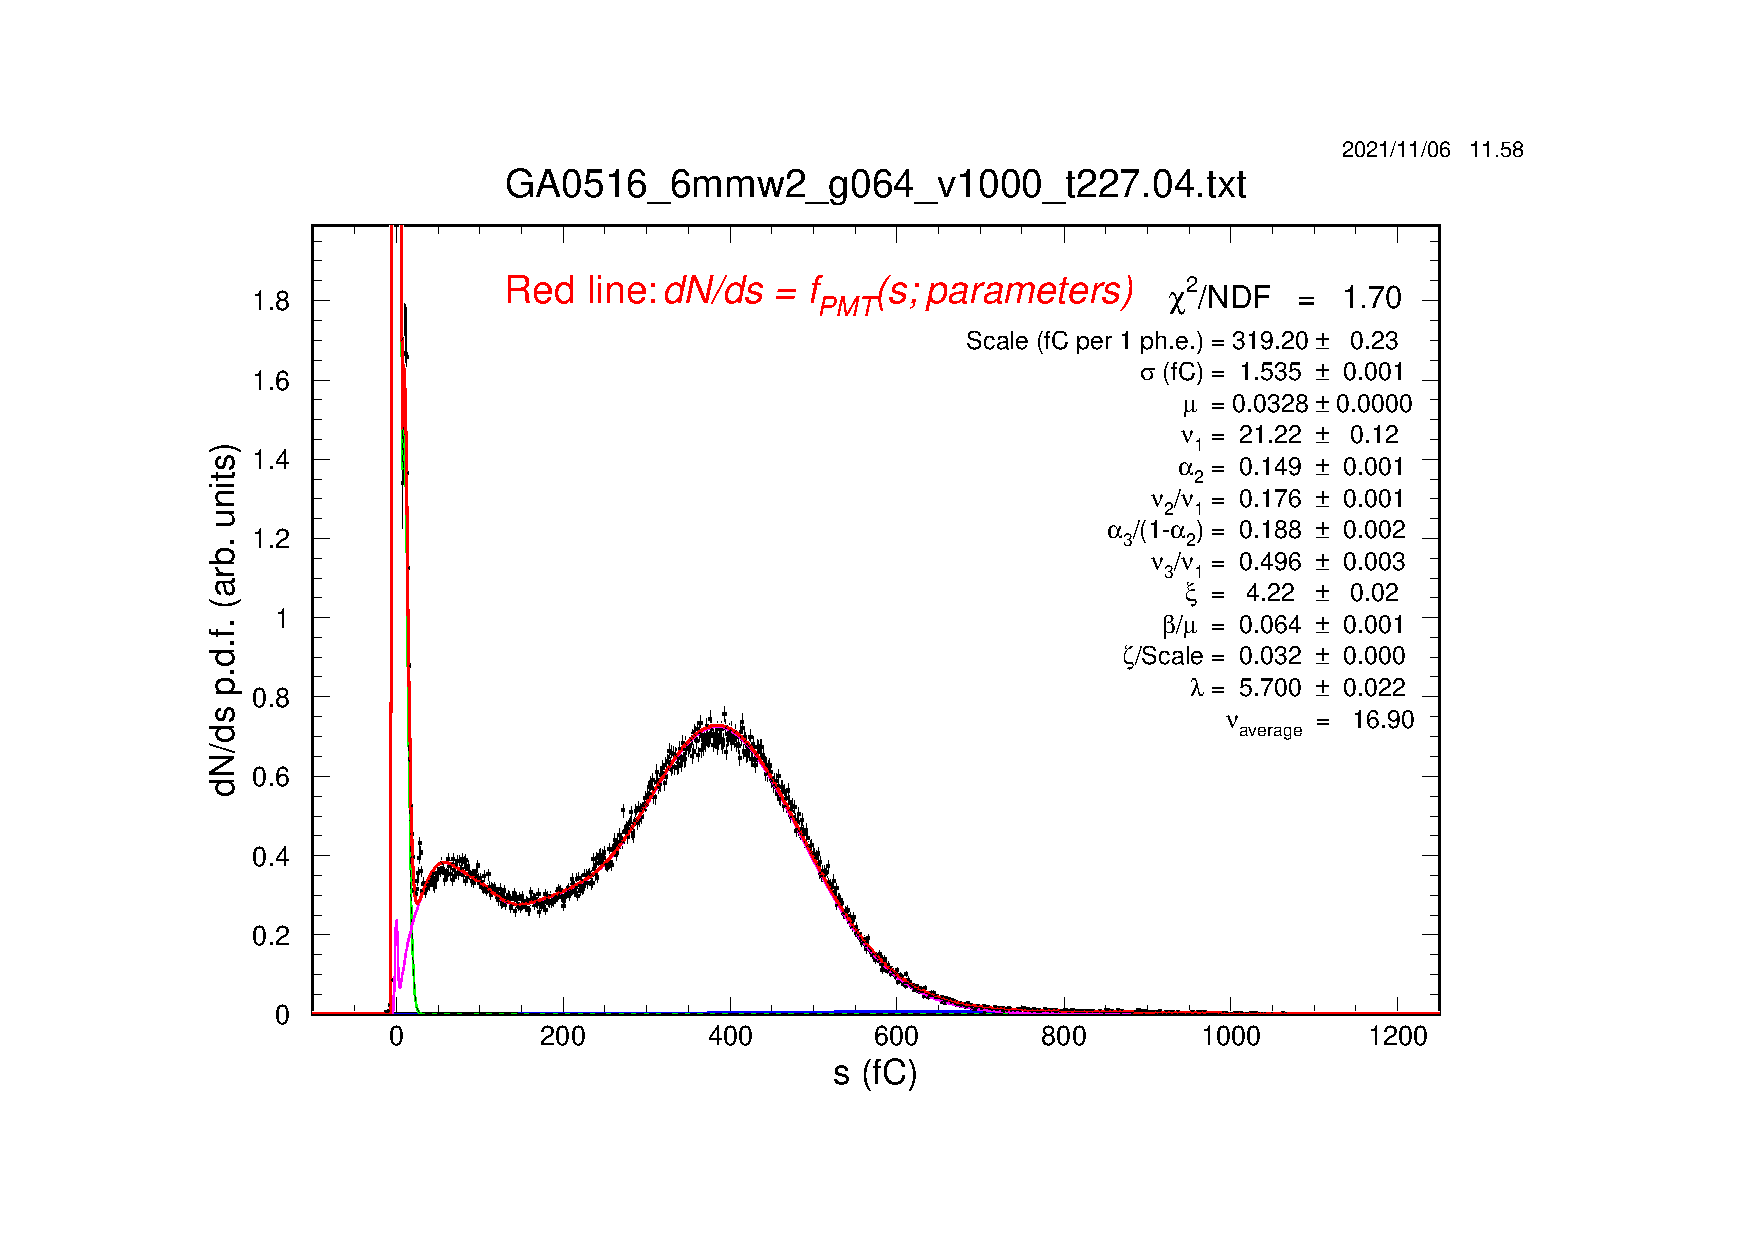
\includegraphics[clip=true,trim=100 75 140 100,width=.49\textwidth,height=.25\textwidth]
                    {figures/GA0516_1c.pdf}}
  \subfloat[No mask, cross talk approximated by fit]{%
    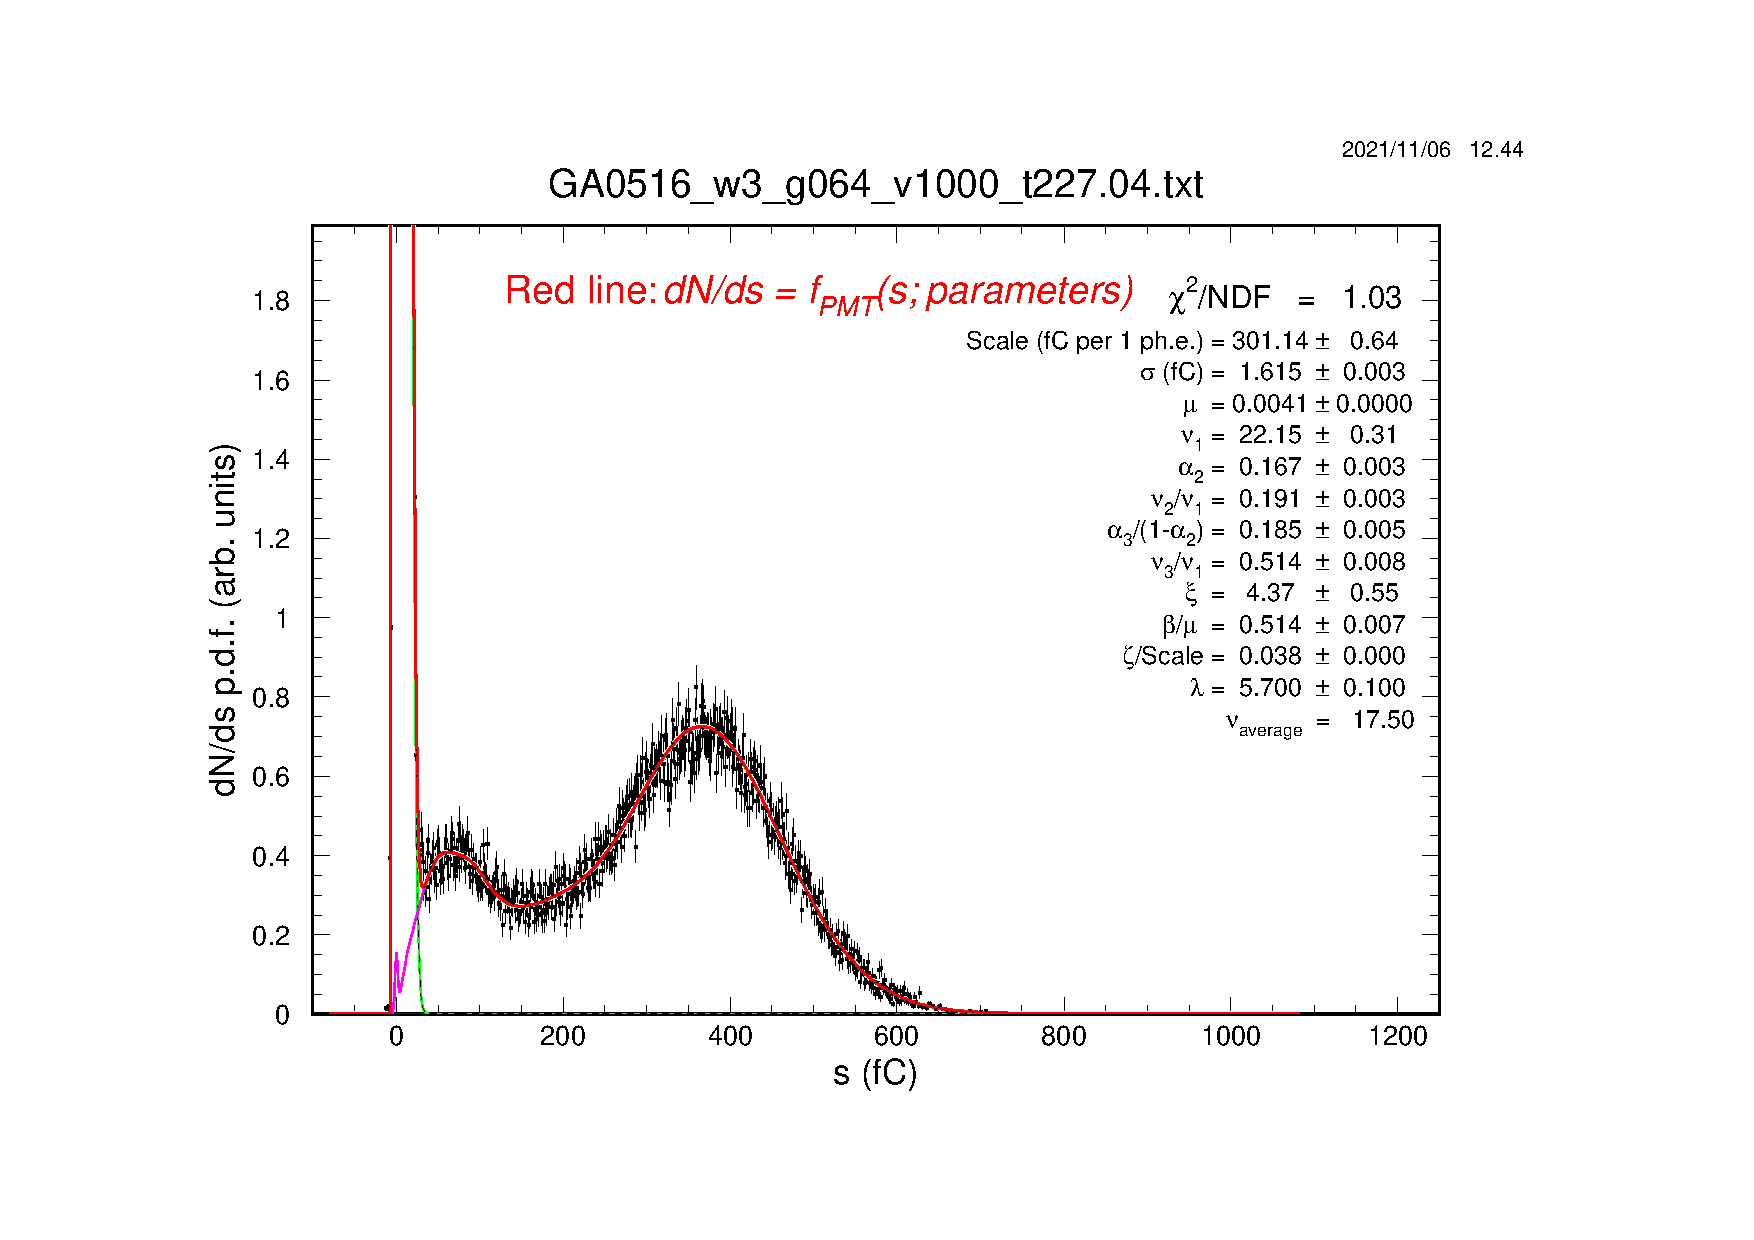
\includegraphics[clip=true,trim=100 75 140 100,width=.49\textwidth,height=.25\textwidth]
                    {figures/GA0516_1d.pdf}}
  \caption{Signal amplitude probability distributions for PMT GA0516 (H12700), pixel 4, at HV = 1000 V. Notation similar to Fig.~\ref{fig:CA7811}. Subplots: (a) 3~mm mask; (b) 6~mm mask; (c) run with full PMT face open with the crosstalk events removed by the correlation analysis; (d) run with full PMT face open with the contribution to the spectrum from the crosstalk events approximated and parameterized by the analysis algorithm.
    }
\label{fig:GA0516_1}
\end{figure*}
\begin{figure*}[h!bt] 
\centering 
  \subfloat[3 mm mask]{%
    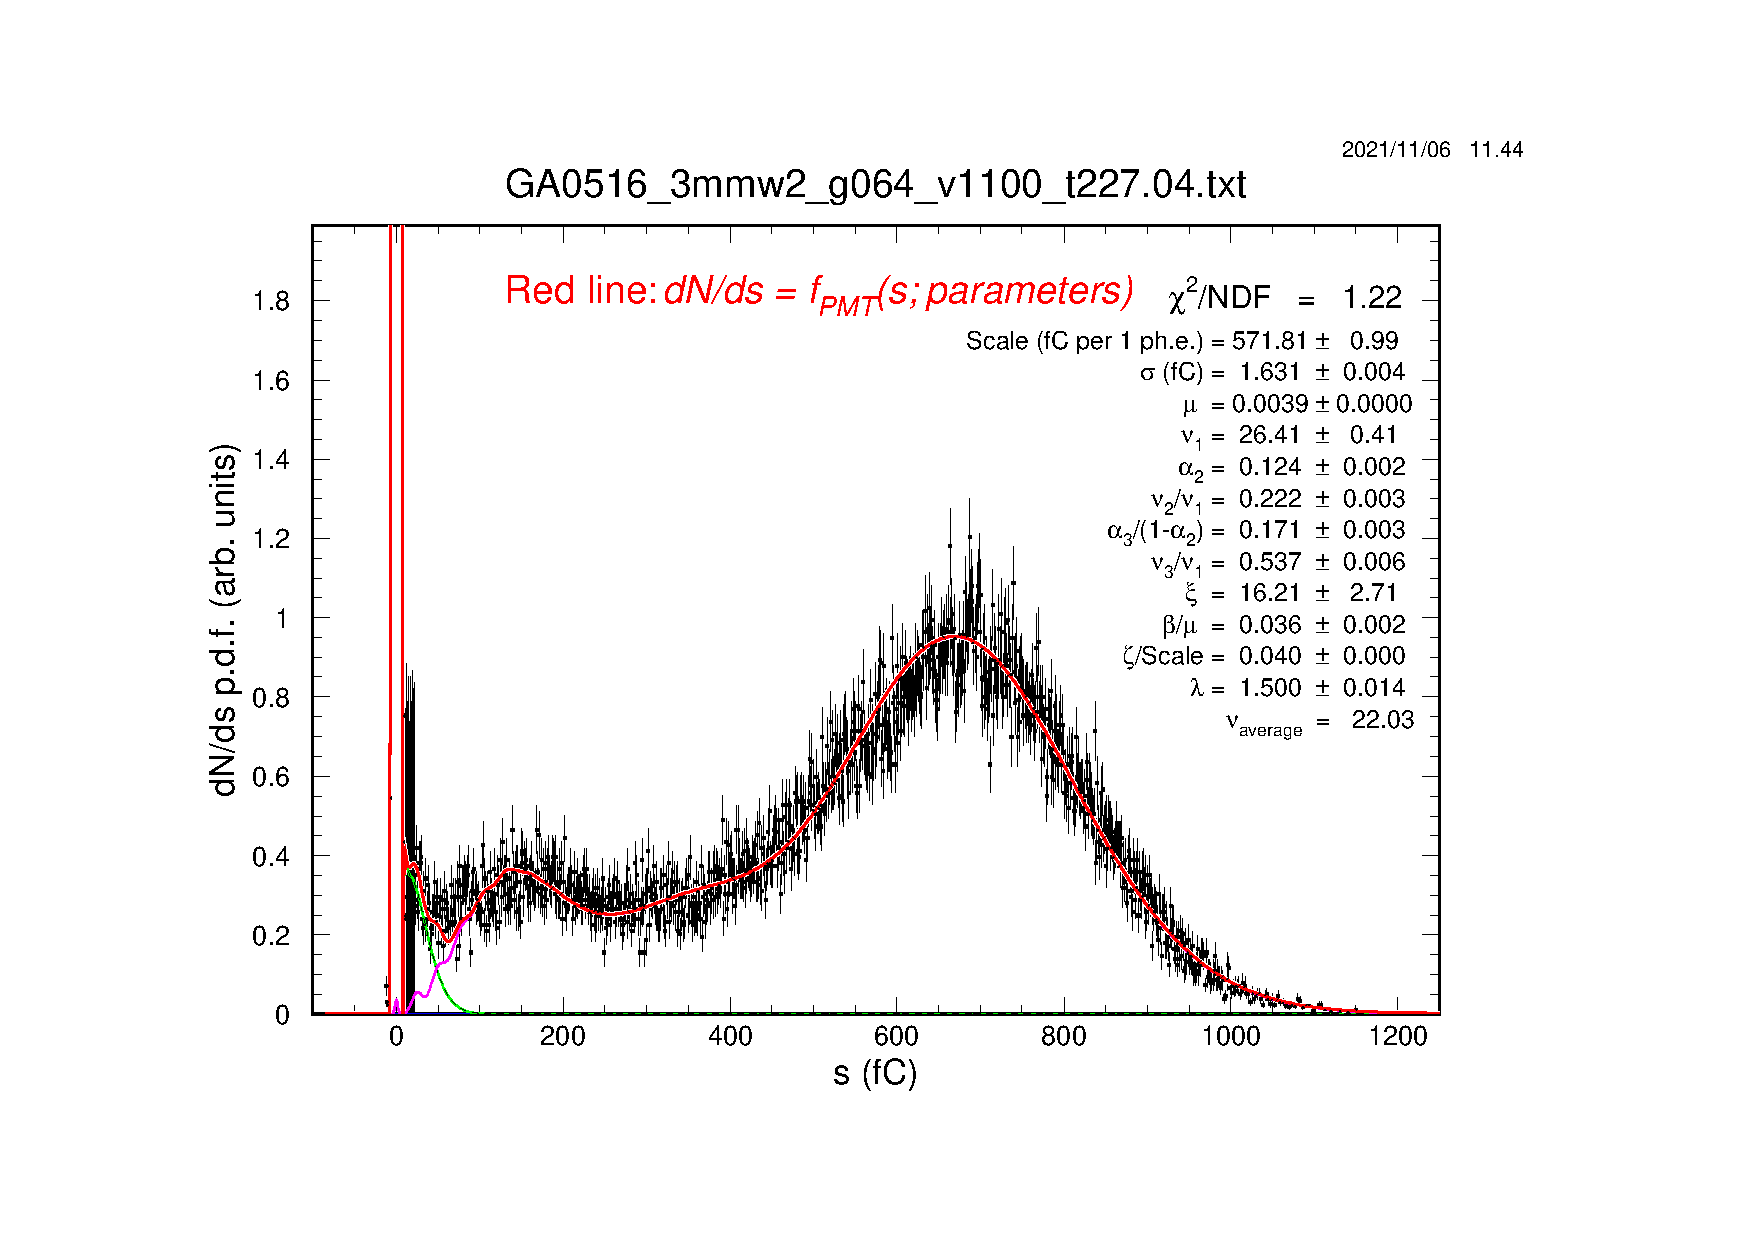
\includegraphics[clip=true,trim=100 75 140 100,width=.49\textwidth,height=.25\textwidth]
                    {figures/GA0516_2a.pdf}}
  \subfloat[6 mm mask]{%
    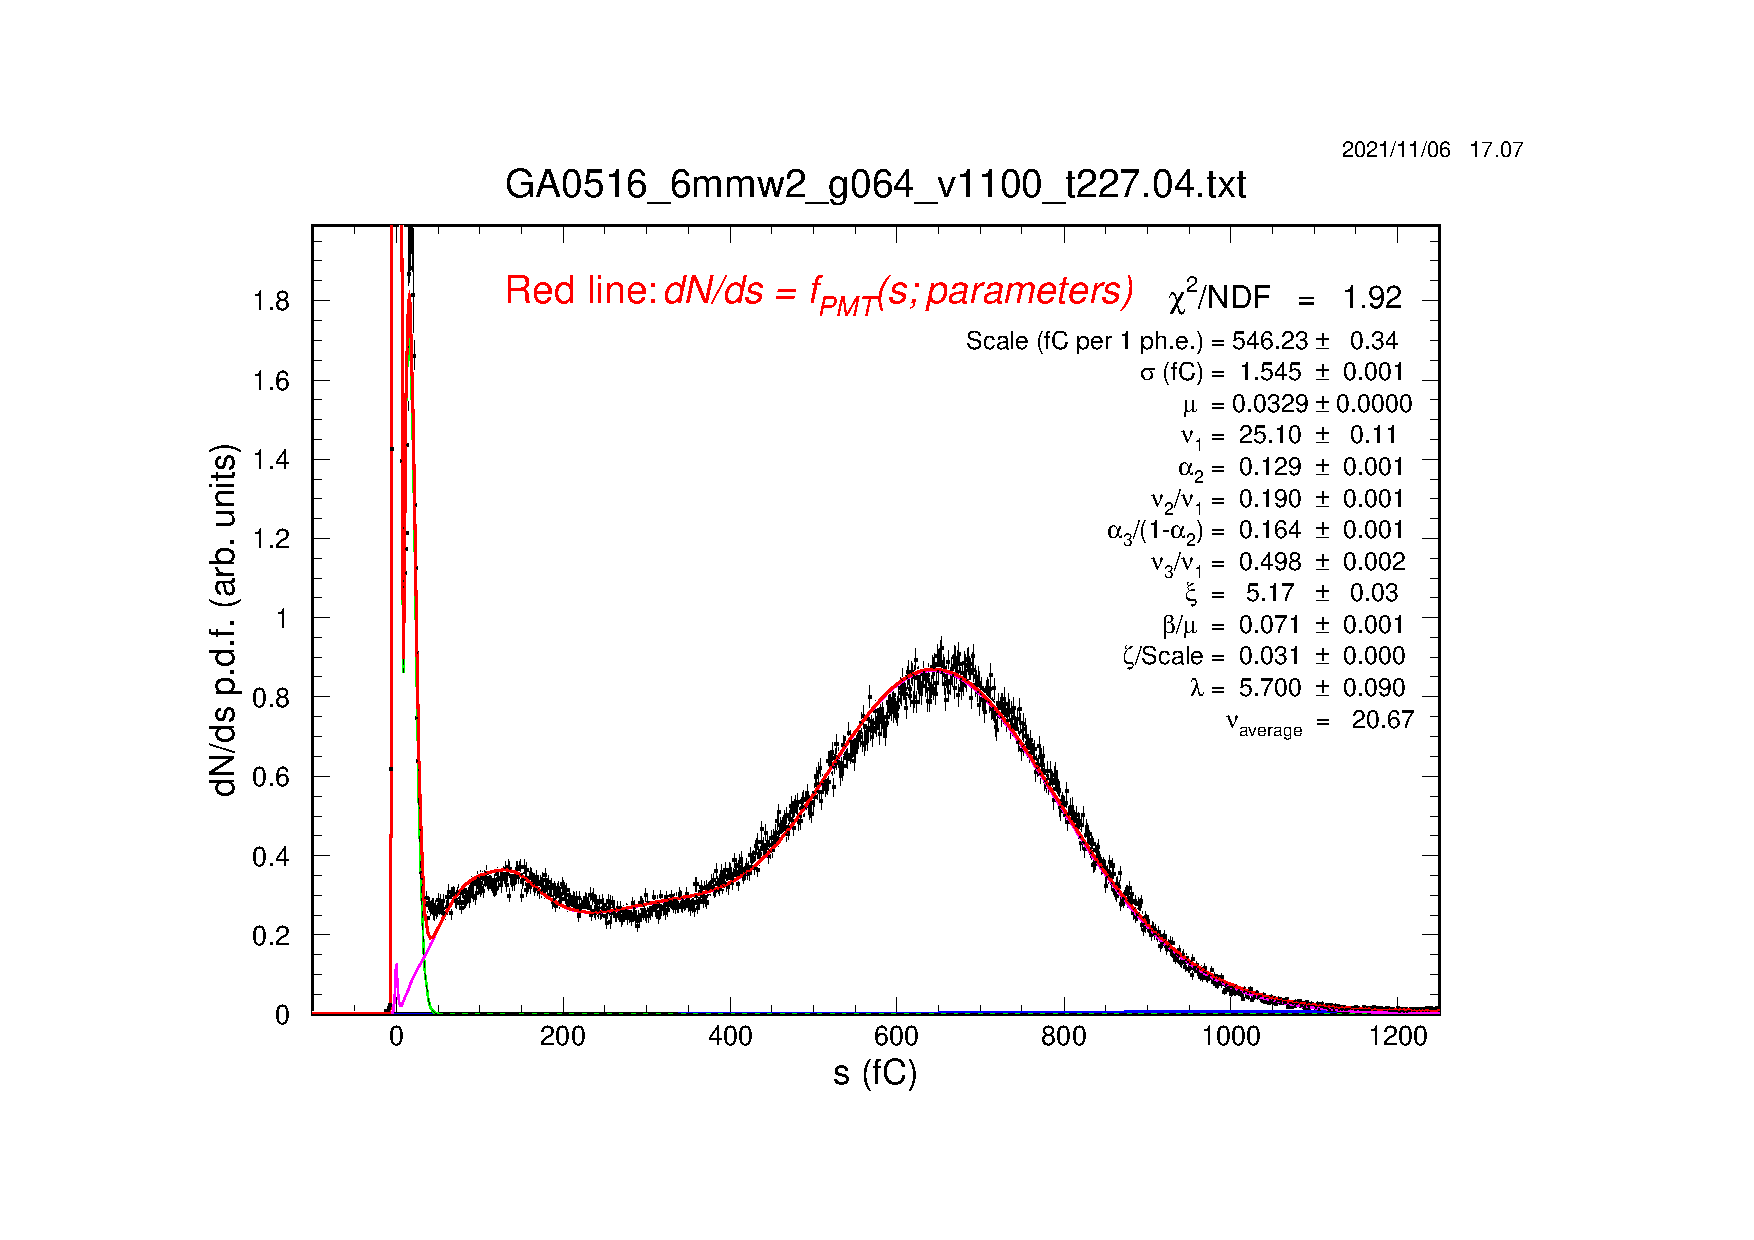
\includegraphics[clip=true,trim=100 75 140 100,width=.49\textwidth,height=.25\textwidth]
                    {figures/GA0516_2b.pdf}} \\
  \subfloat[No mask, cross talk removed by software]{%
    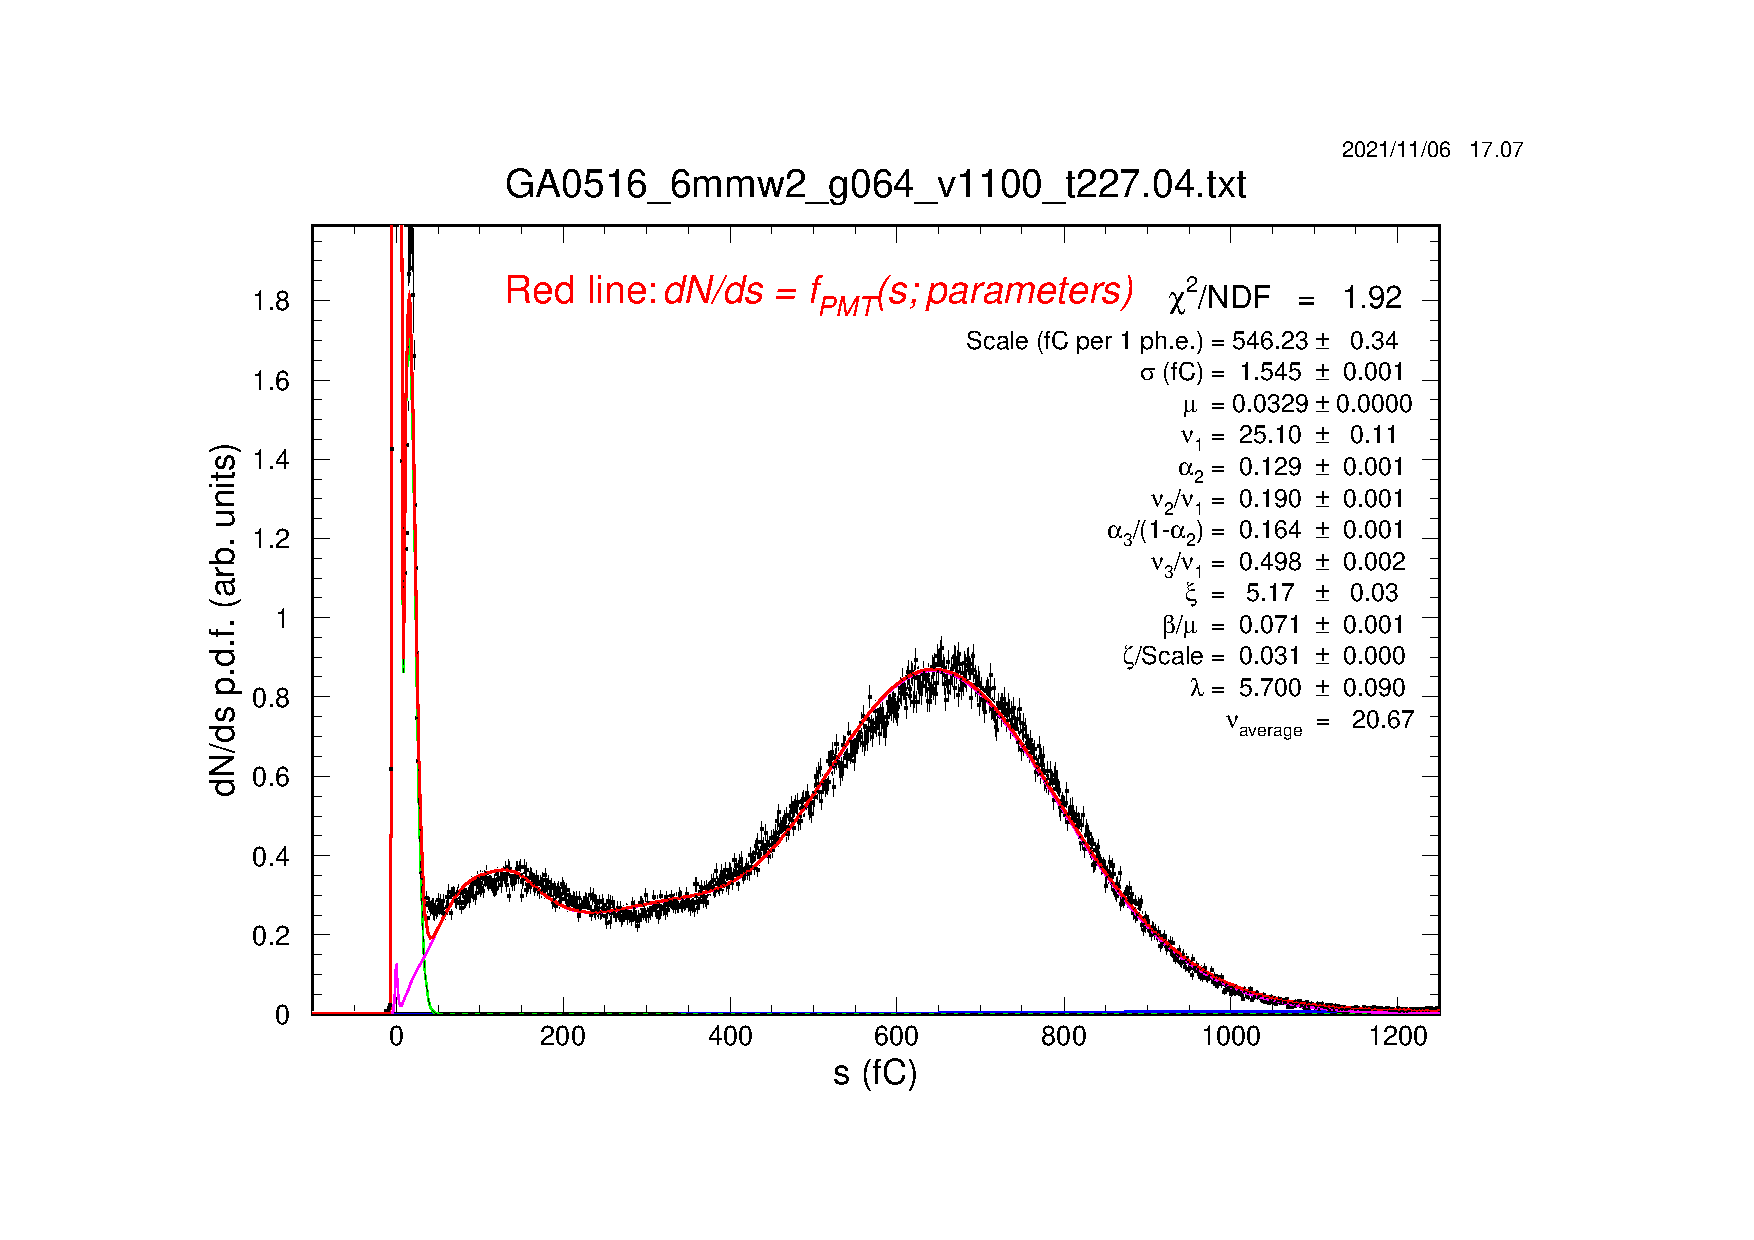
\includegraphics[clip=true,trim=100 75 140 100,width=.49\textwidth,height=.25\textwidth]
                    {figures/GA0516_2c.pdf}}
  \subfloat[No mask, cross talk approximated by fit]{%
    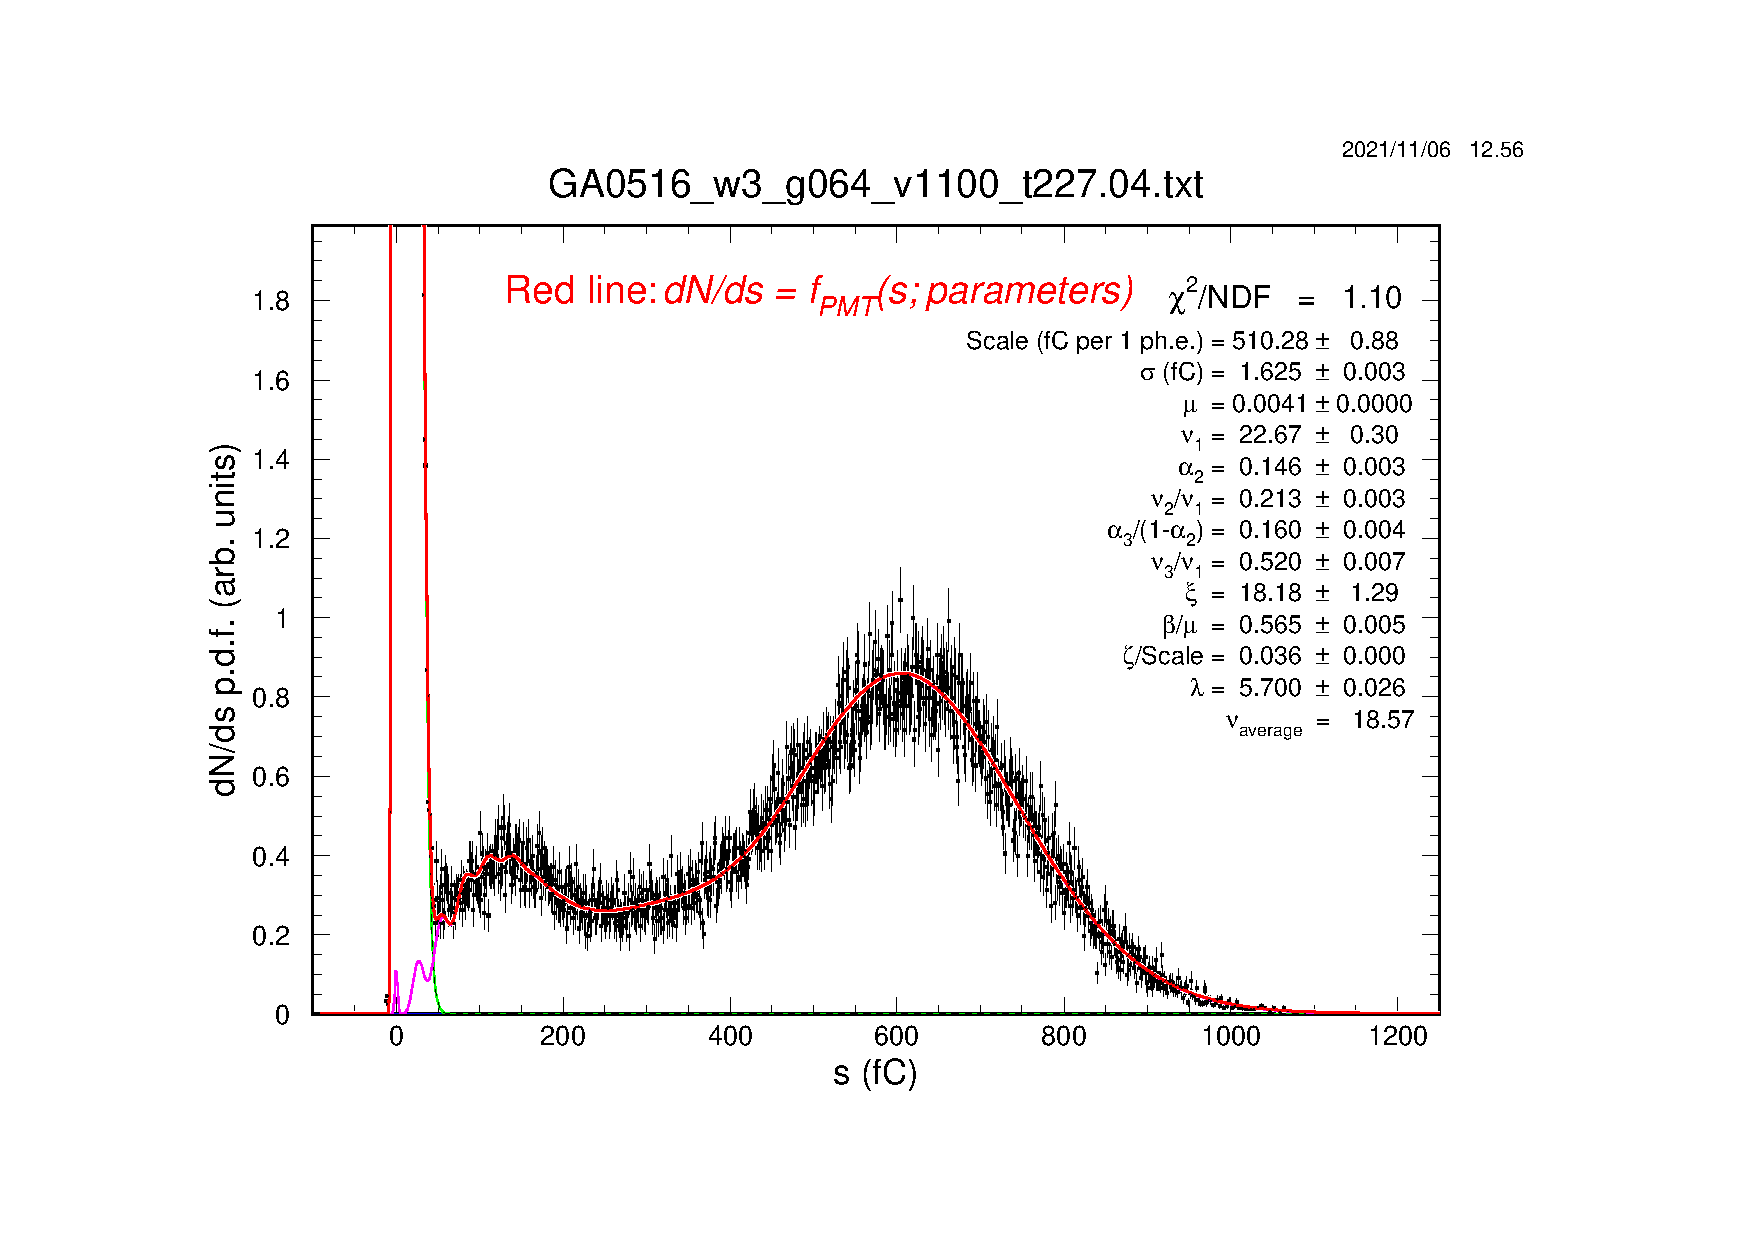
\includegraphics[clip=true,trim=100 75 140 100,width=.49\textwidth,height=.25\textwidth]
                    {figures/GA0516_2d.pdf}}
  \caption{Same as Fig.~\ref{fig:GA0516_1}, but with all the data taken at HV = 1100~V. 
    }
\label{fig:GA0516_2}
\end{figure*}
\begin{figure*}[h!bt] 
\centering 
  \subfloat[6 mm mask, at HV = 1000 V]{%
    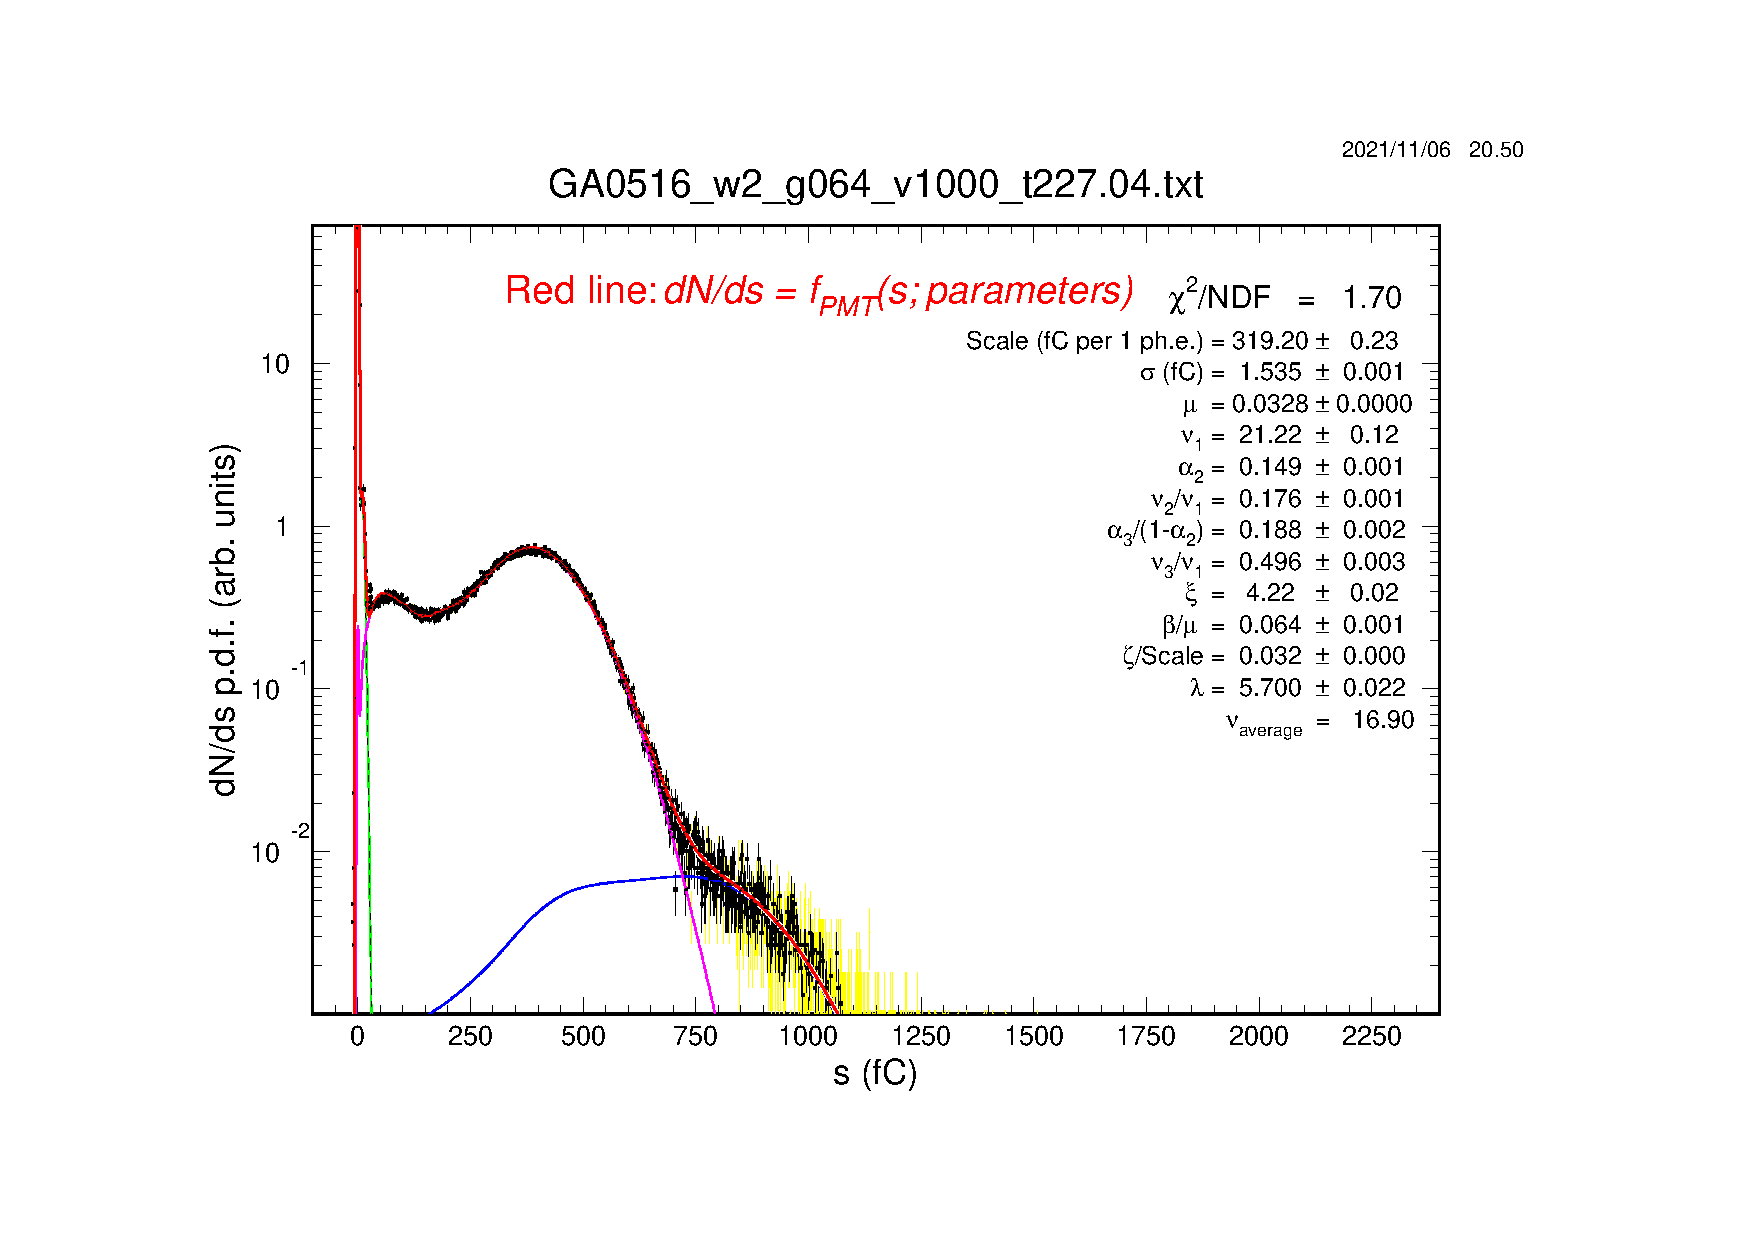
\includegraphics[clip=true,trim=100 75 140 100,width=.49\textwidth,height=.24\textwidth]
                    {figures/GA0516_3a.pdf}}
  \subfloat[6 mm mask, at HV = 1100 V]{%
    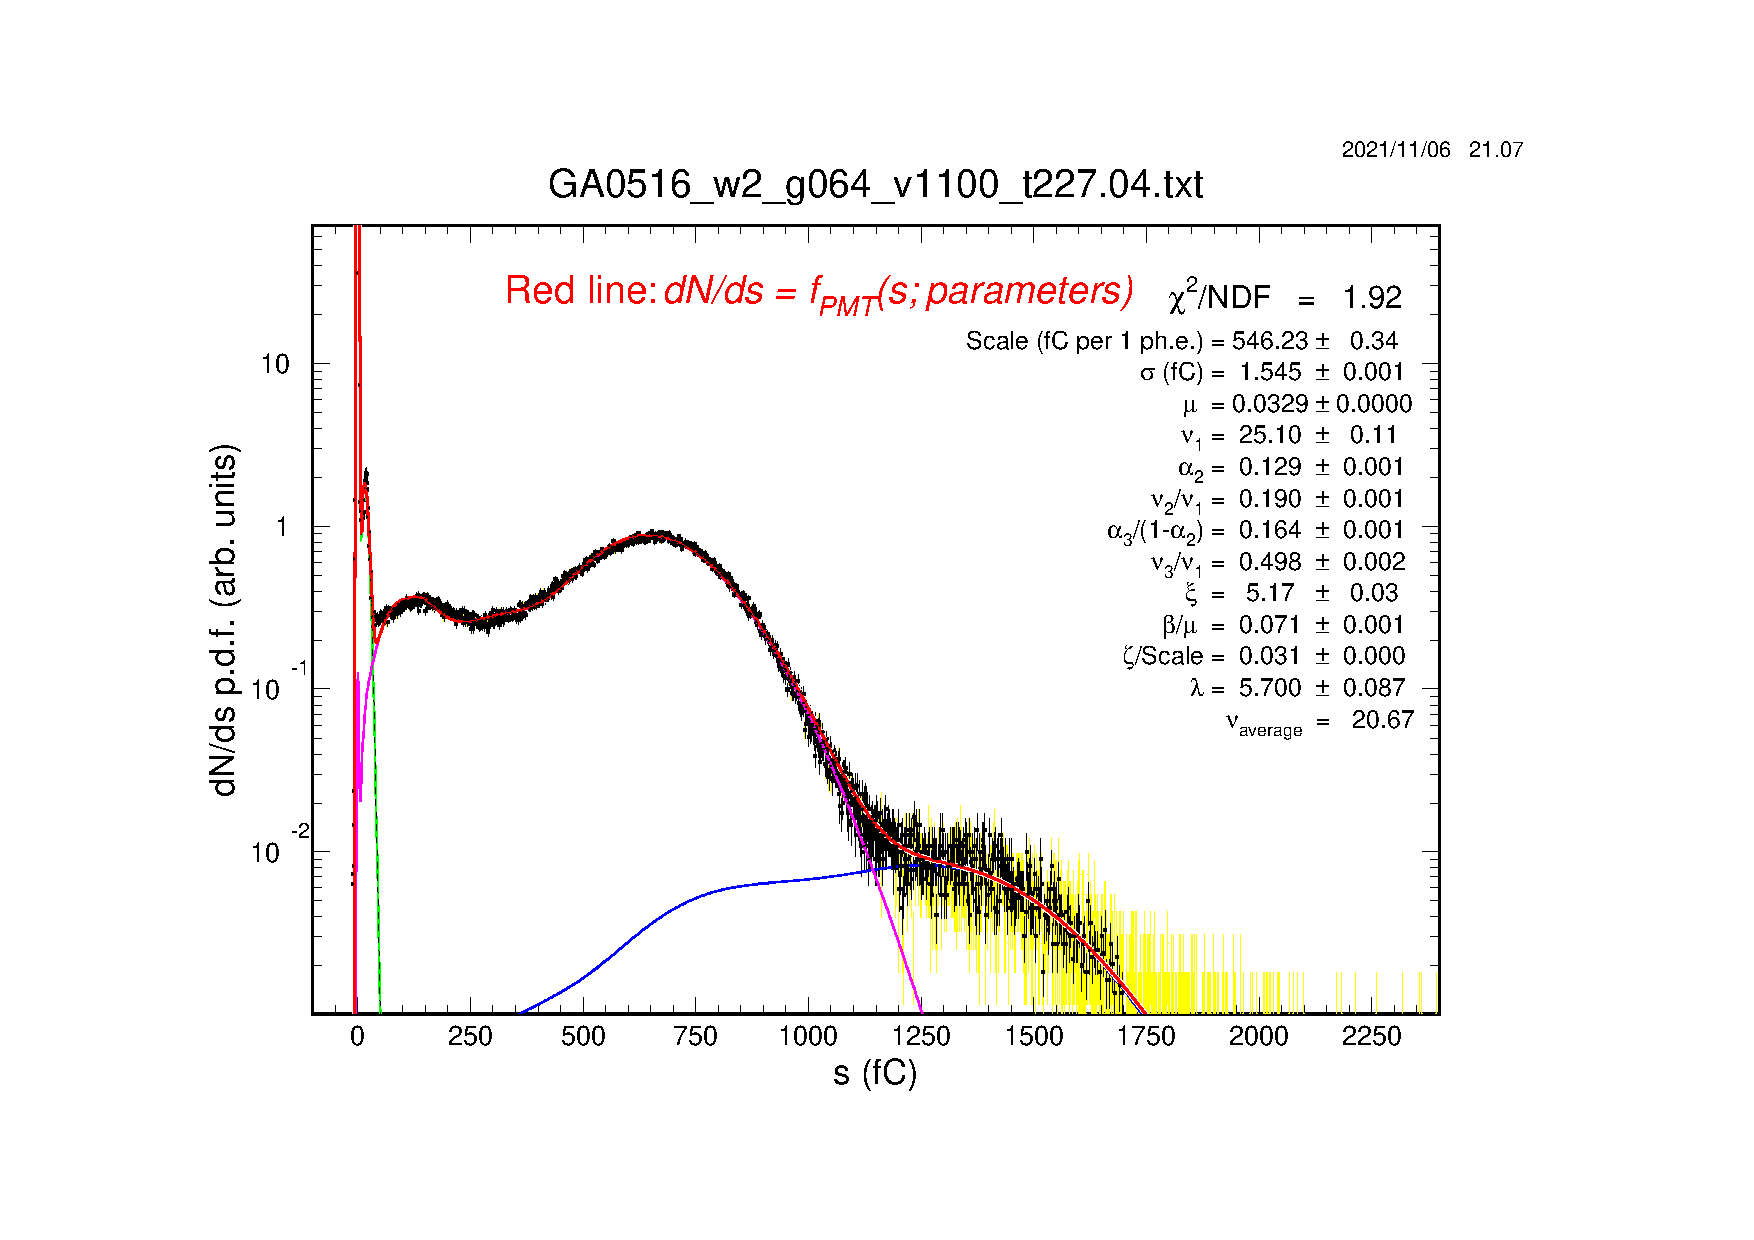
\includegraphics[clip=true,trim=100 75 140 100,width=.49\textwidth,height=.24\textwidth]
                    {figures/GA0516_3b.pdf}} \\
  \subfloat[No mask, at HV = 1000 V]{%
    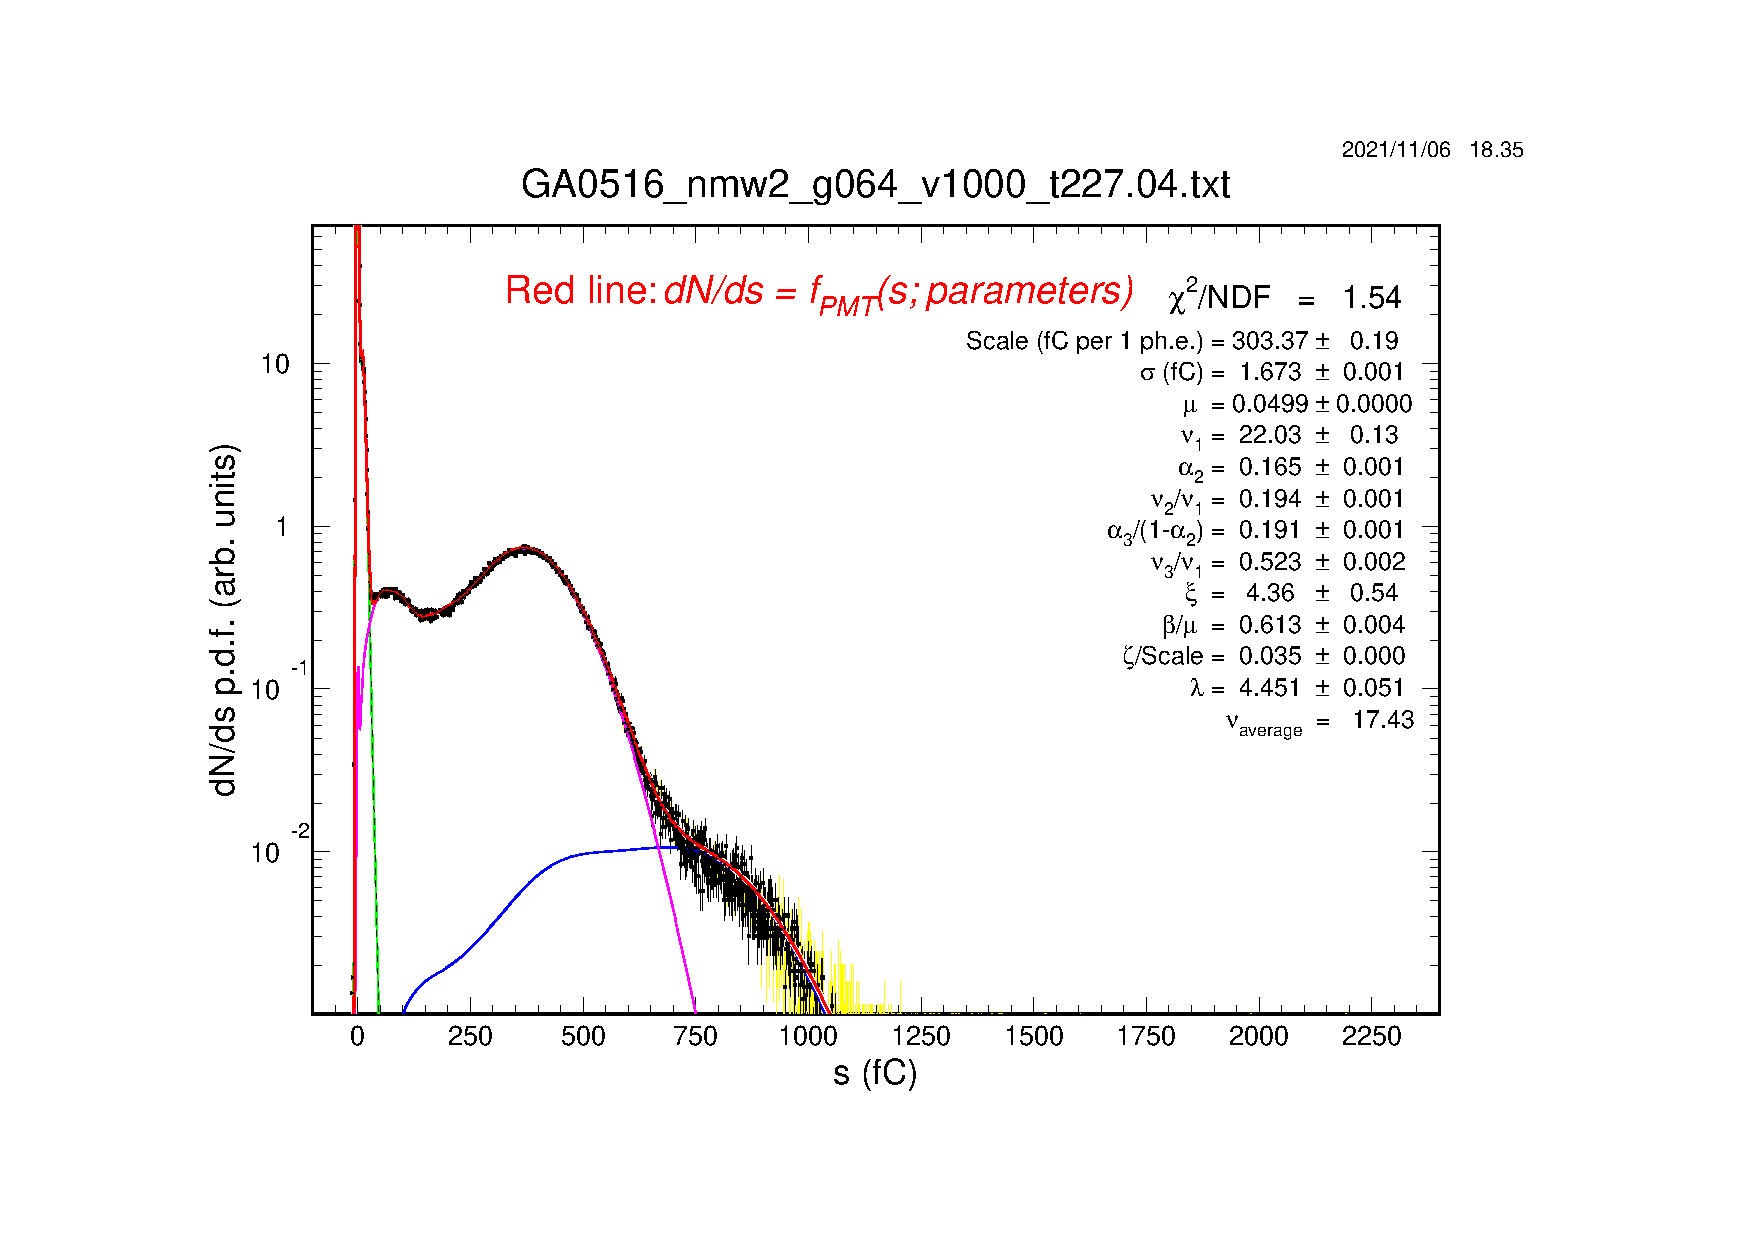
\includegraphics[clip=true,trim=100 75 140 100,width=.49\textwidth,height=.24\textwidth]
                    {figures/GA0516_3c.pdf}}
  \subfloat[No mask, at HV = 1100 V]{%
    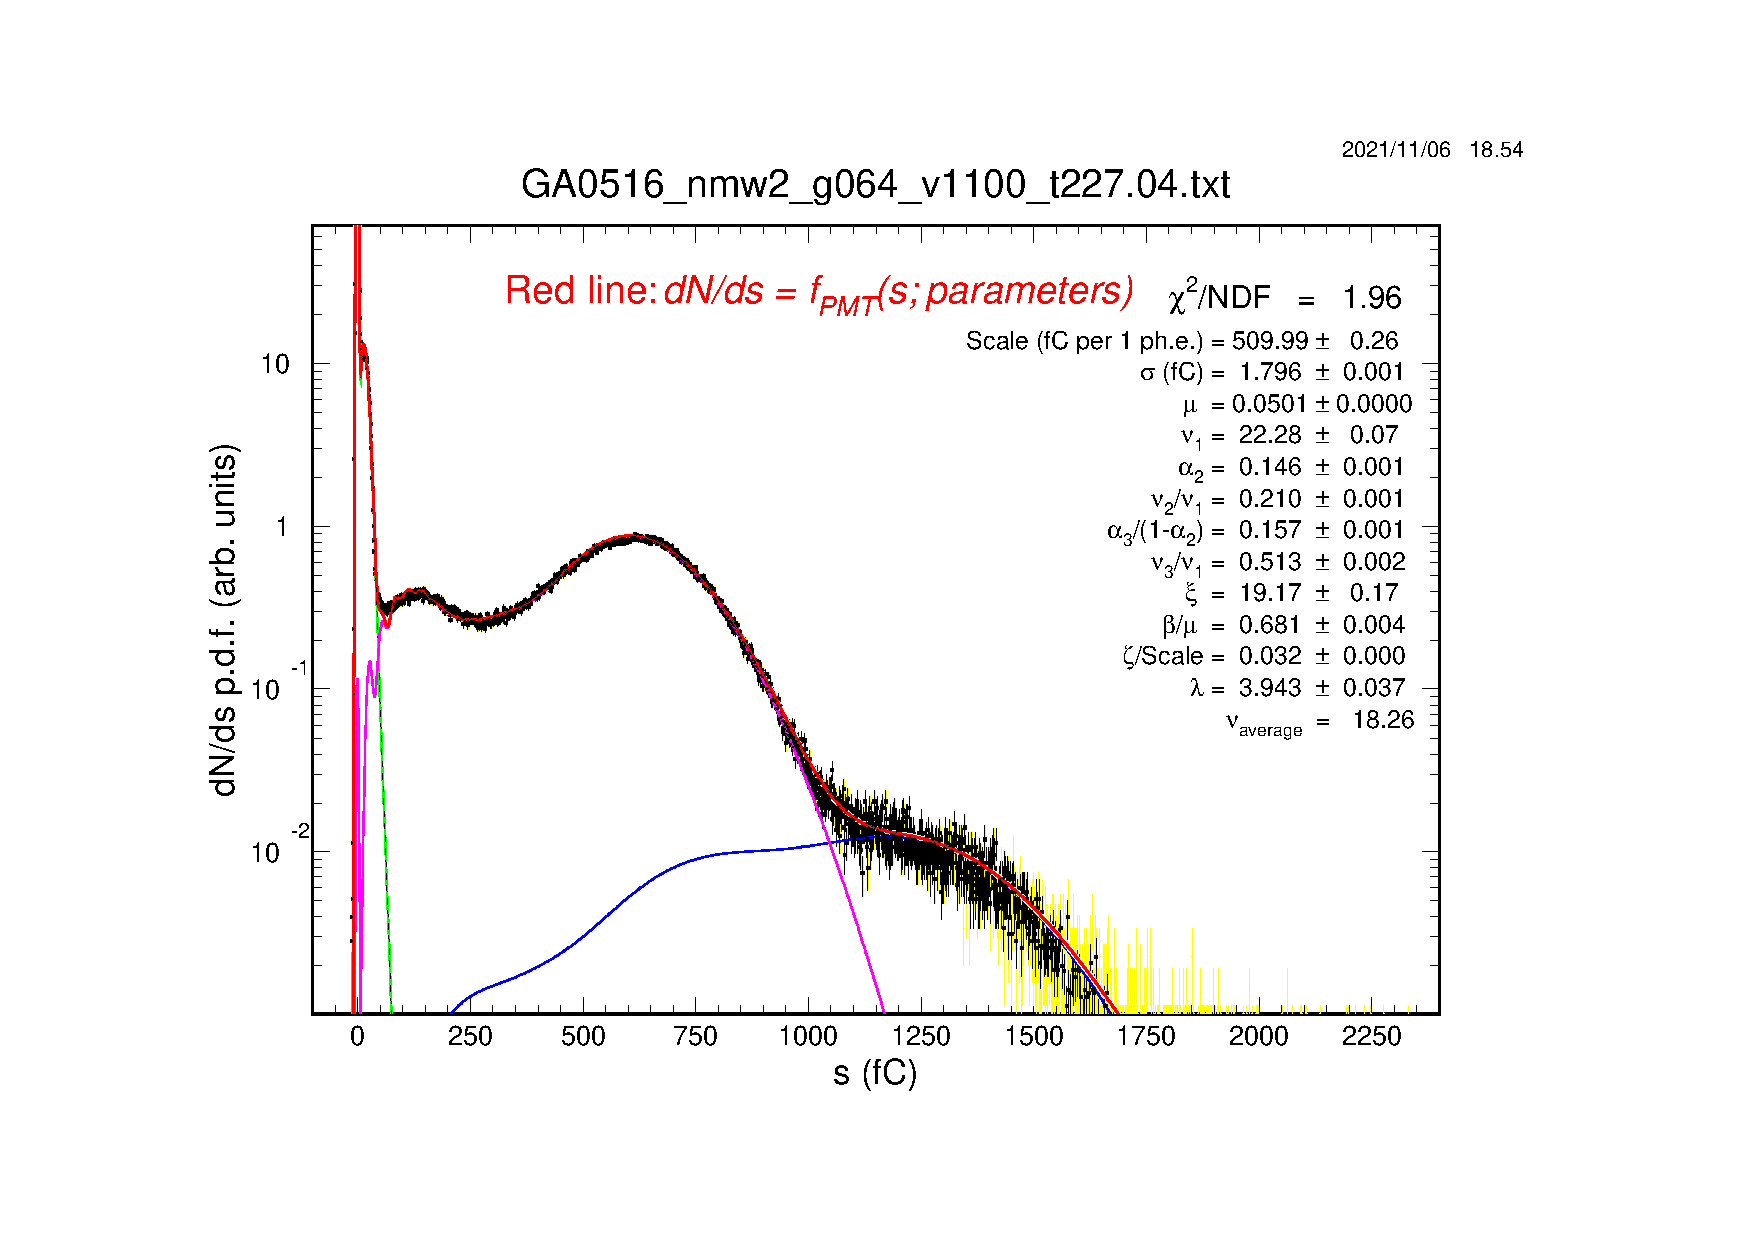
\includegraphics[clip=true,trim=100 75 140 100,width=.49\textwidth,height=.24\textwidth]
                    {figures/GA0516_3d.pdf}}
  \caption{Signal amplitude probability distributions for PMT GA0516 (H12700), pixel 4, medium light intensity, at HV = 1000 V ((a) and (c)) and at HV = 1100 V ((b) and (d)). Notation similar to Fig.~\ref{fig:CA7811}. To avoid statistical instabilities in the fitting procedure bins with low statistics at high amplitudes (shown by the yellow histogram) were combined and averaged to provide better Gaussian spread (black points with errors).  Subplots: (a) and (b) run with 6 mm mask covering the full PMT face except pixel 4; (c) and (d) run with full PMT face open with the contribution to the spectrum from the crosstalk events approximated and parametrized by the analysis algorithm. Contributions to the spectra are shown by colors: red is the single photoelectron, blue - two or more photoelectrons, green-black dashed line shows the measurement function including the pedestal Gaussian and the crosstalk contribution. 
    }
\label{fig:GA0516_3}
\end{figure*}
\begin{figure*}[h!bt] 
\centering 
  \subfloat[6 mm mask, at HV = 1000 V]{%
    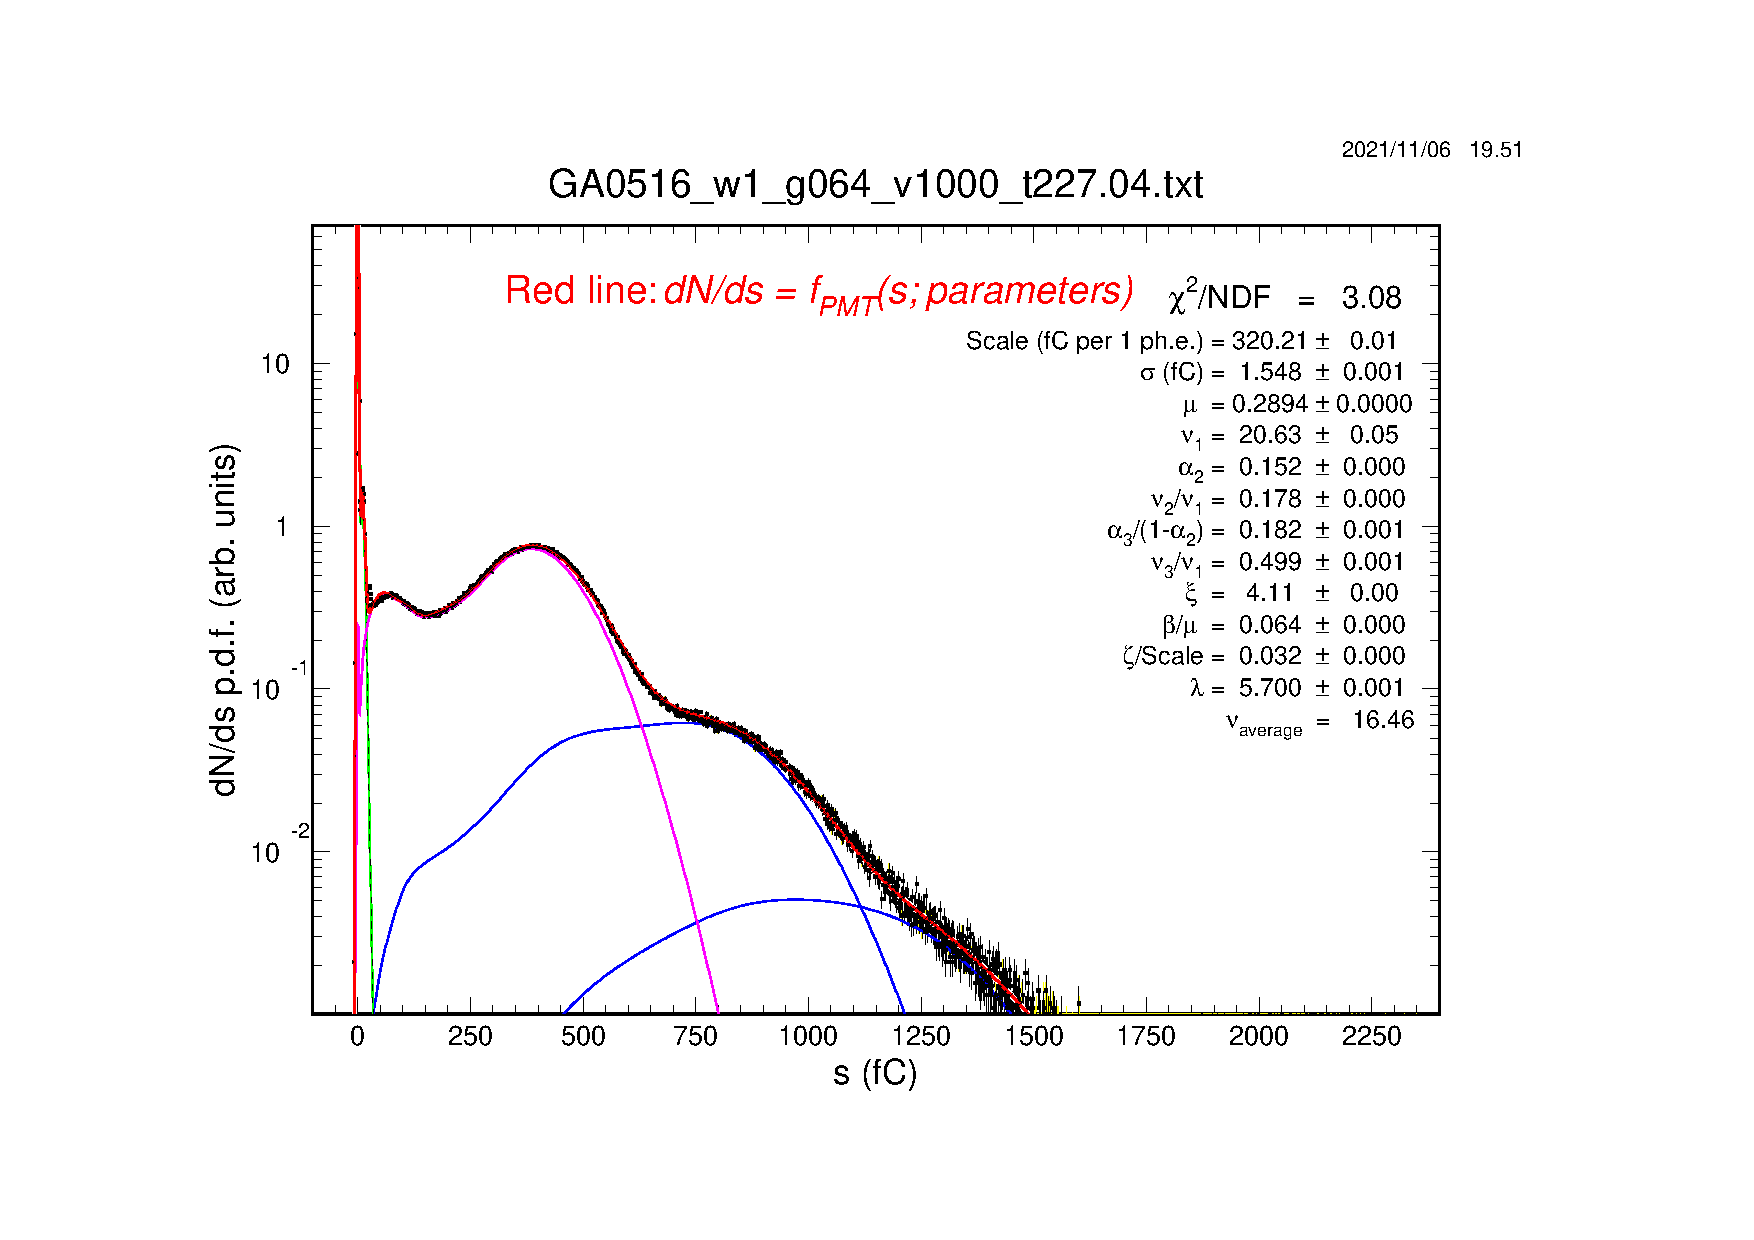
\includegraphics[clip=true,trim=100 75 140 100,width=.49\textwidth,height=.24\textwidth]
                    {figures/GA0516_4a.pdf}}
  \subfloat[6 mm mask, at HV = 1100 V]{%
    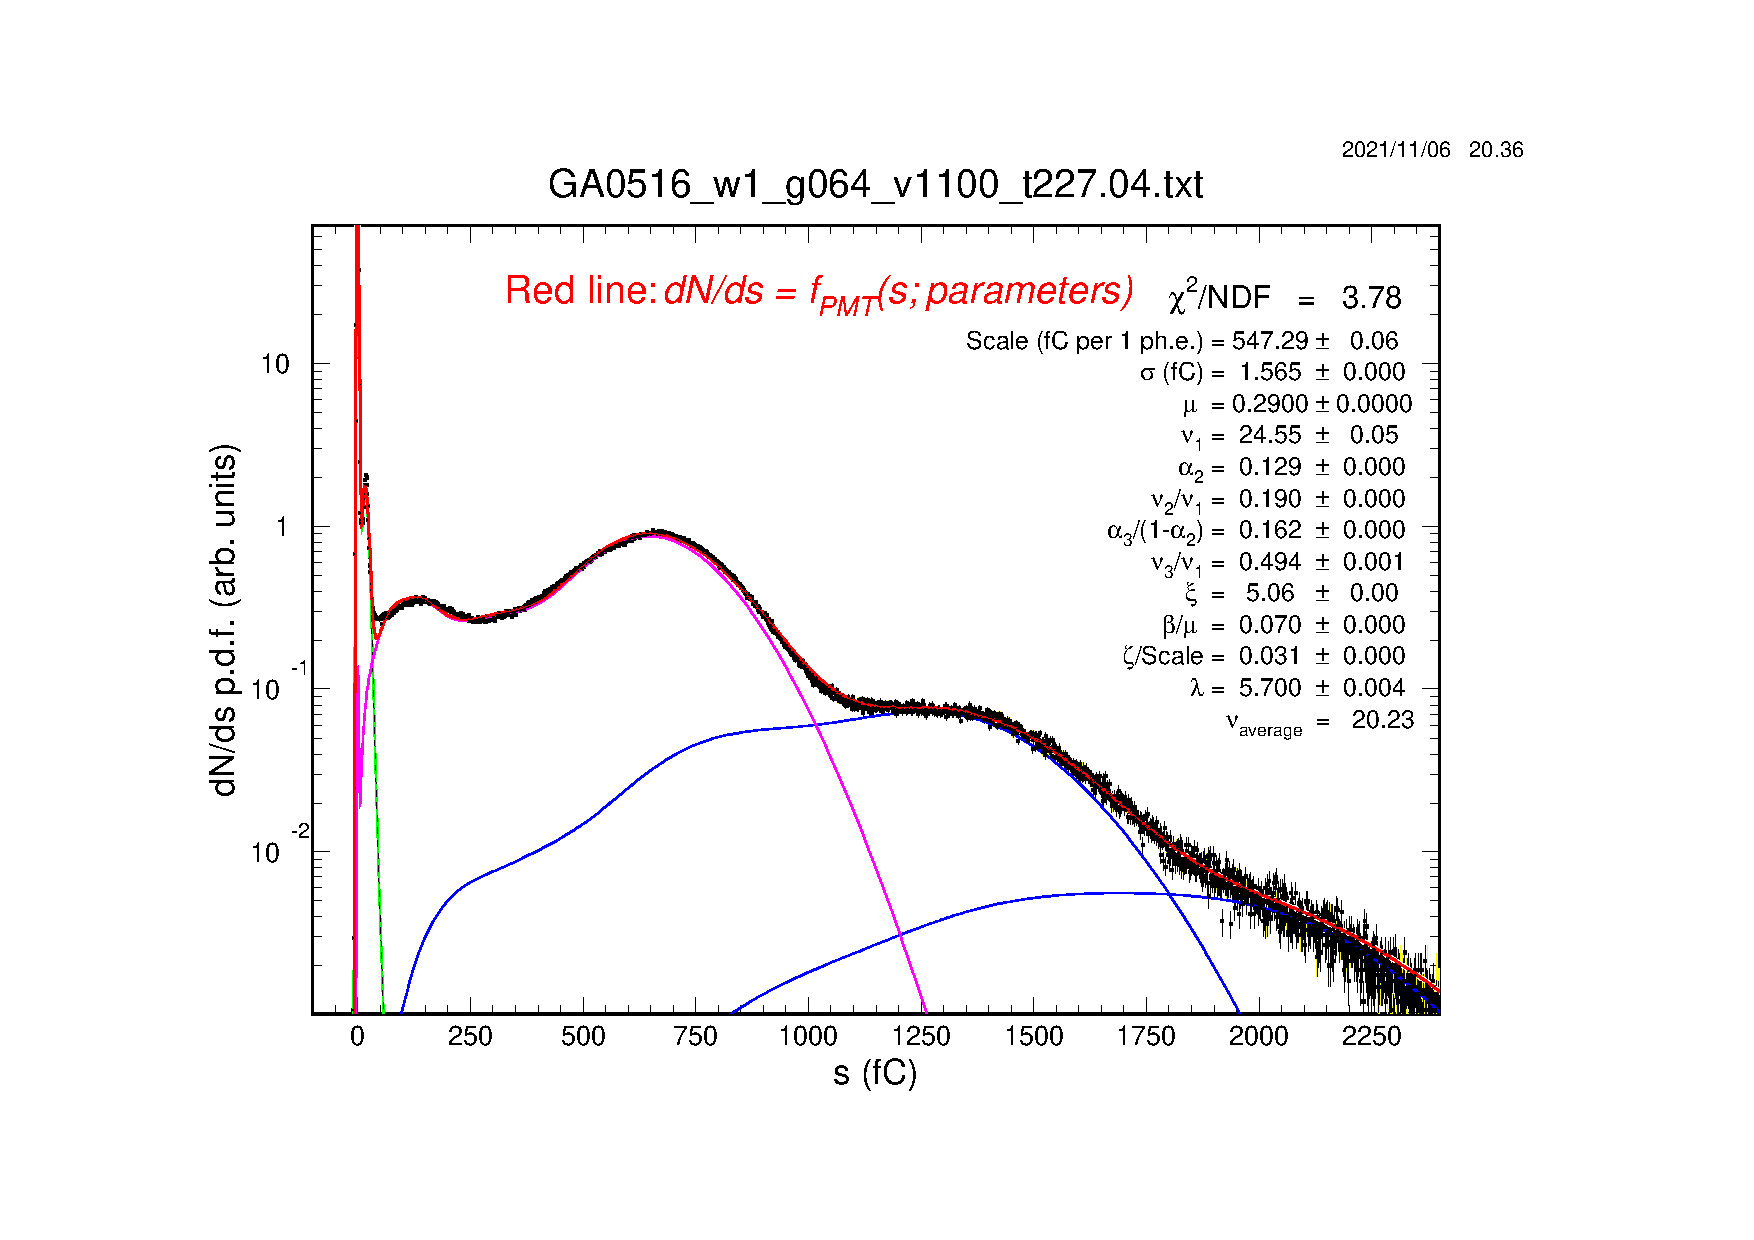
\includegraphics[clip=true,trim=100 75 140 100,width=.49\textwidth,height=.24\textwidth]
                    {figures/GA0516_4b.pdf}} \\
  \subfloat[No mask, at HV = 1000 V]{%
    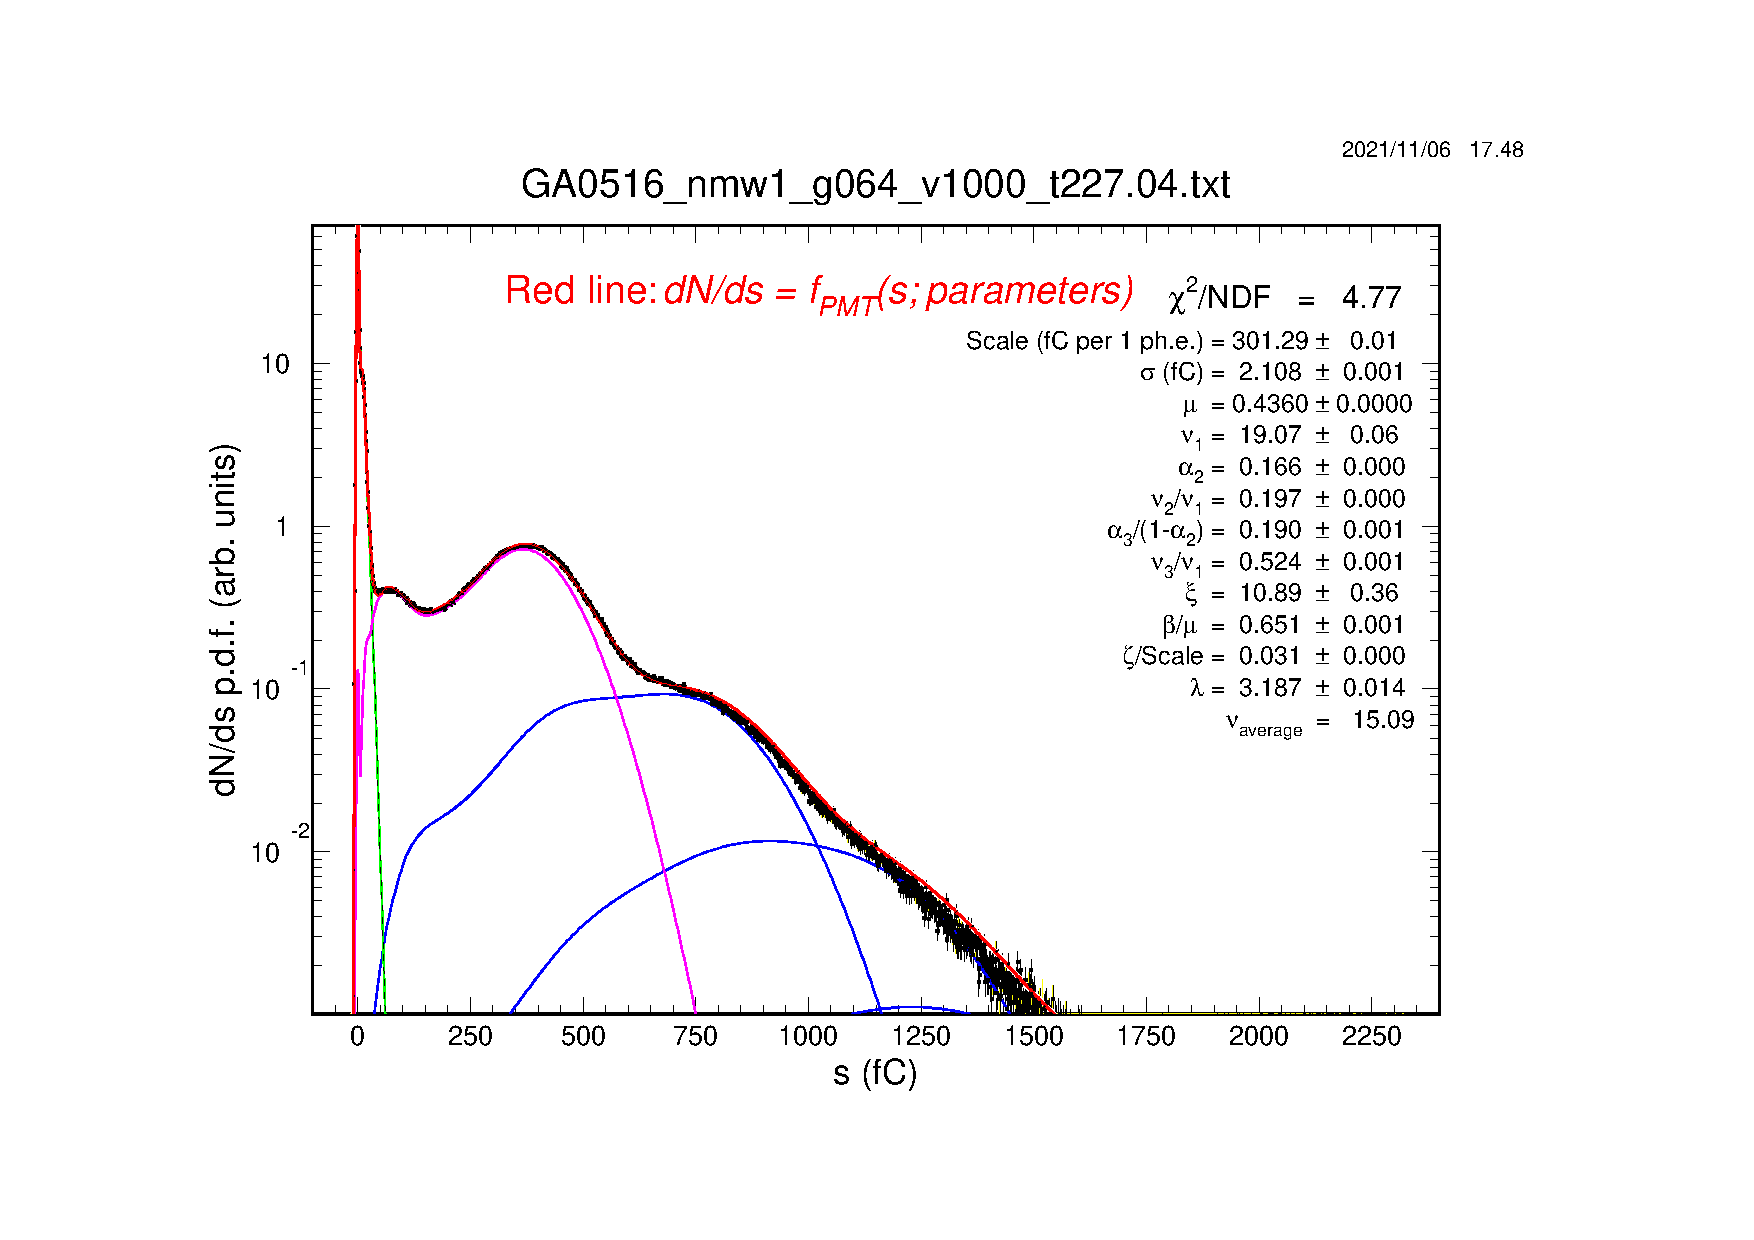
\includegraphics[clip=true,trim=100 75 140 100,width=.49\textwidth,height=.24\textwidth]
                    {figures/GA0516_4c.pdf}}
  \subfloat[No mask, at HV = 1100 V]{%
    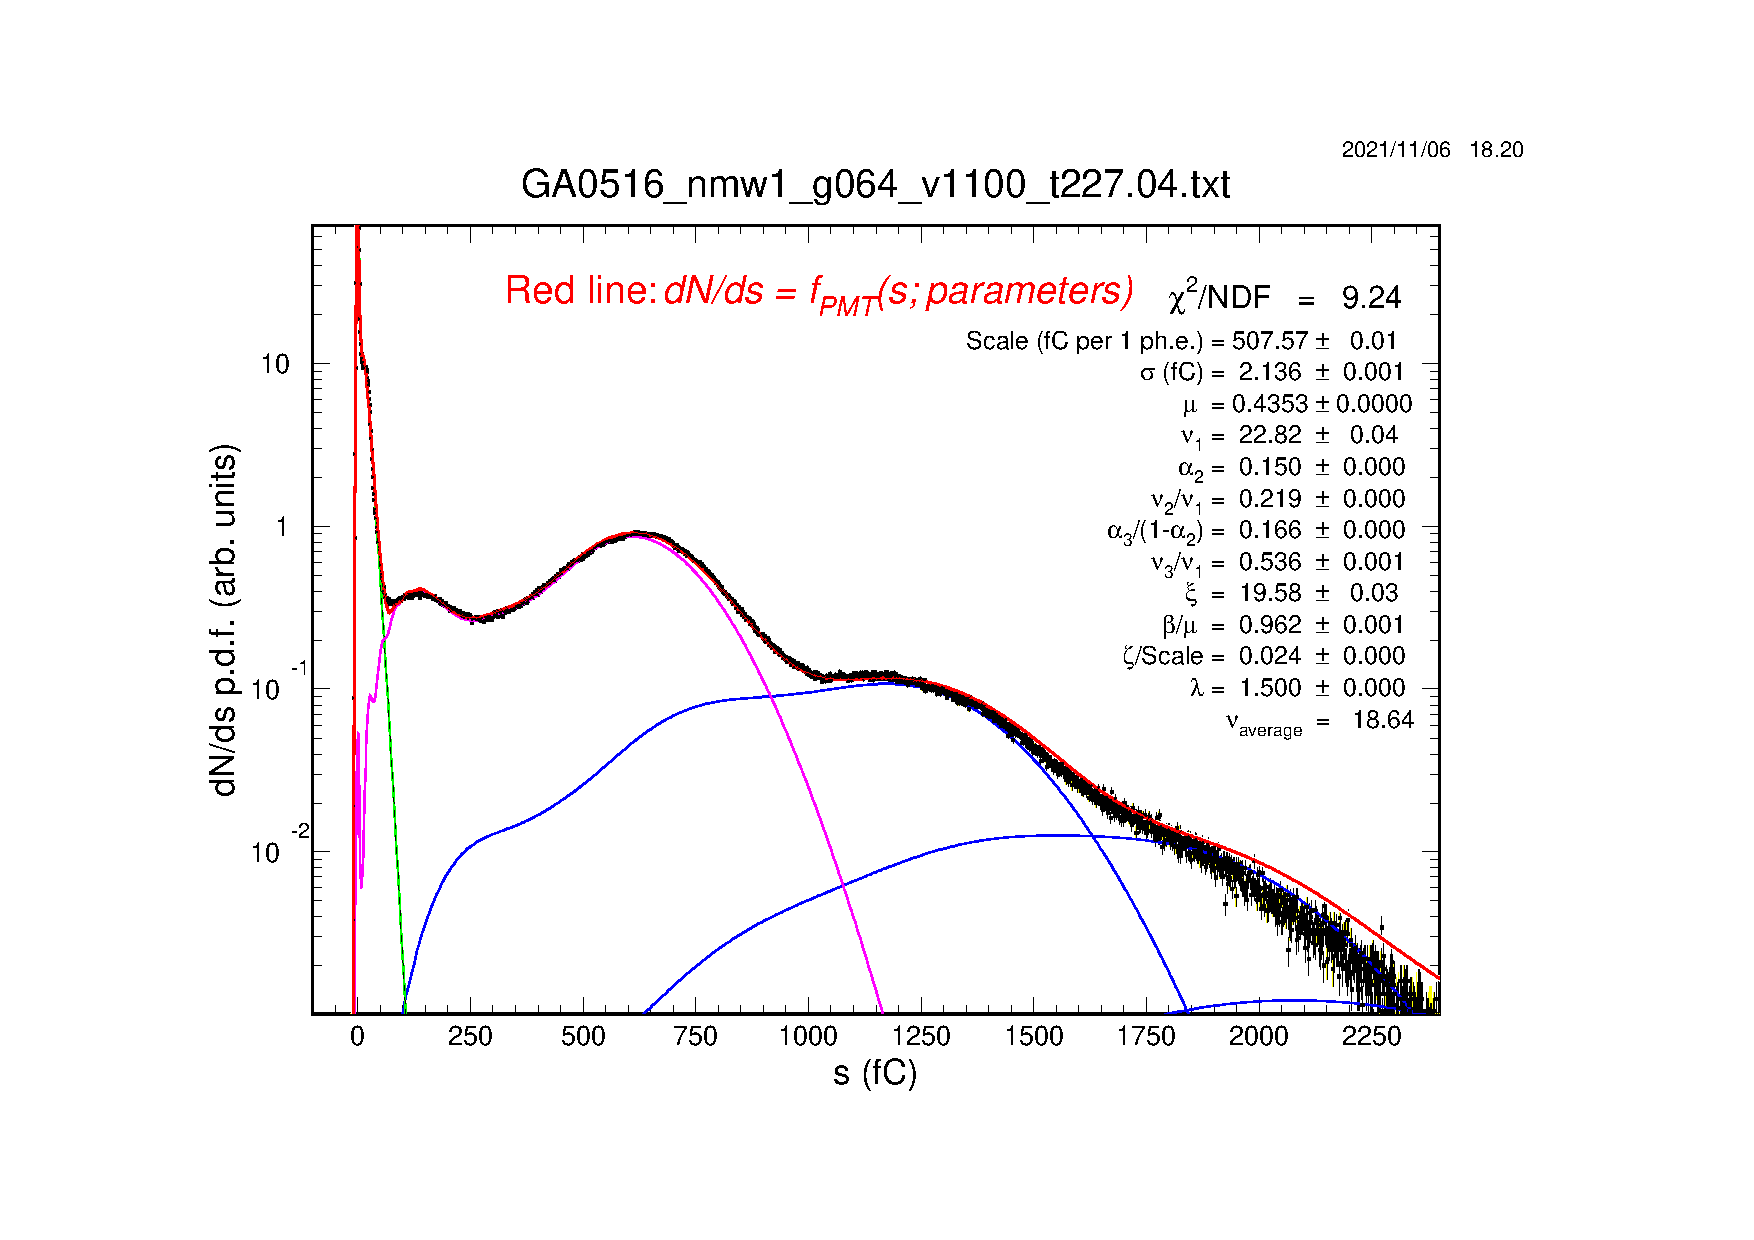
\includegraphics[clip=true,trim=100 75 140 100,width=.49\textwidth,height=.24\textwidth]
                    {figures/GA0516_4d.pdf}}
  \caption{Same as Fig.~\ref{fig:GA0516_3}, but at highest light intensity.
    }
\label{fig:GA0516_4}
\end{figure*}


\begin{figure*}[!ht]
	\centering
	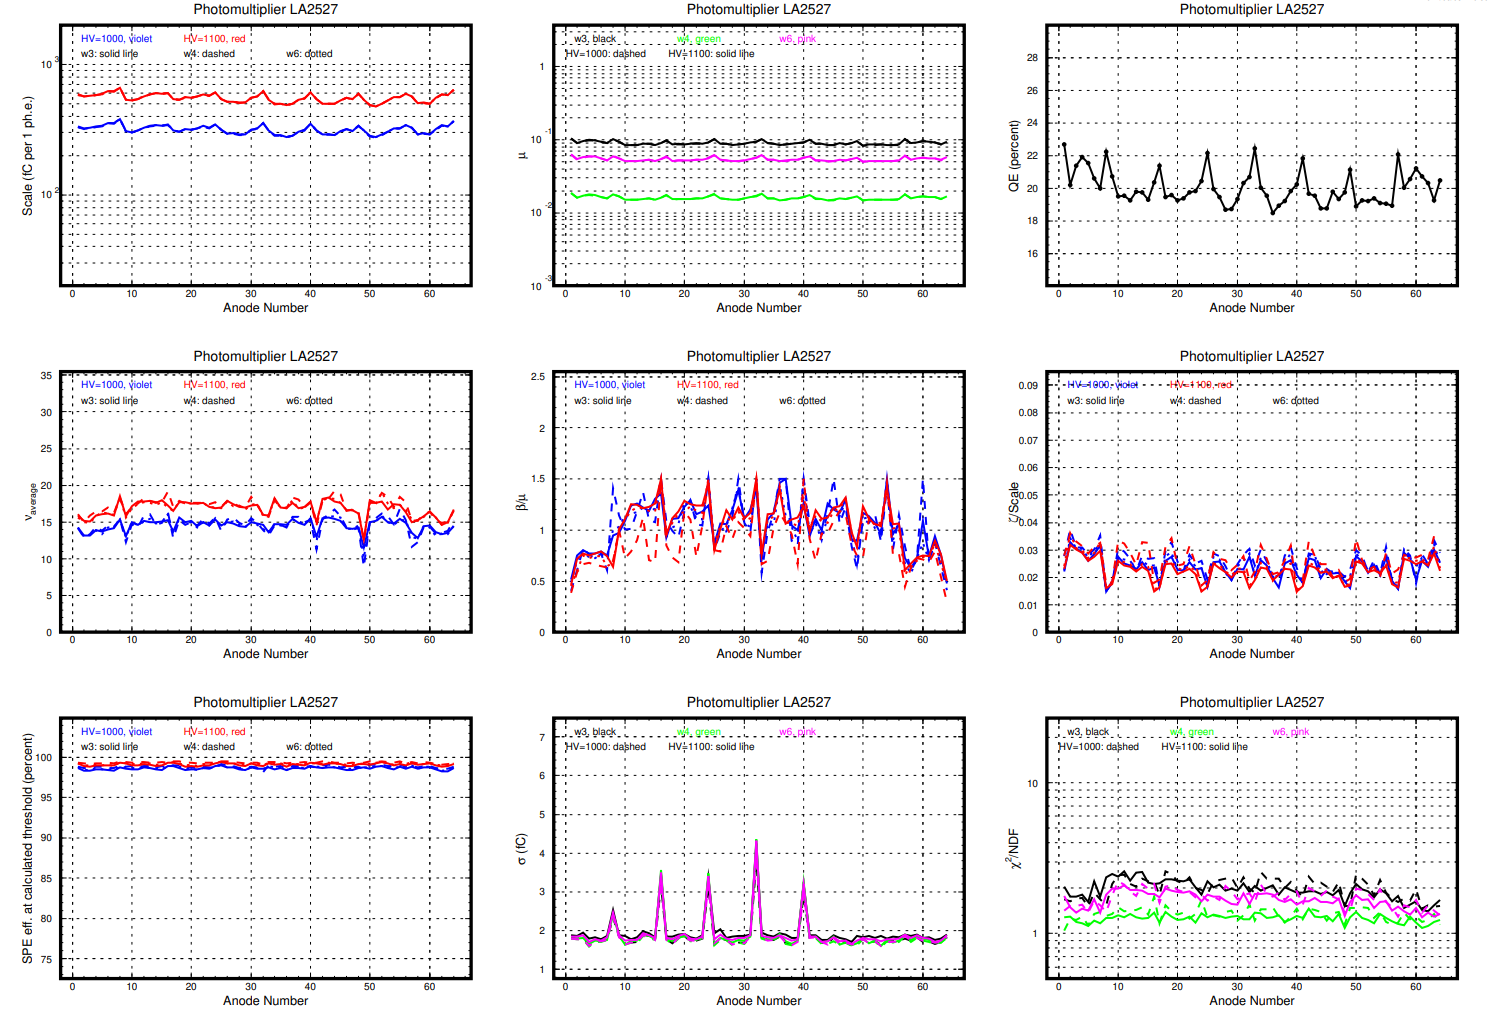
\includegraphics[width=1.0\textwidth,height=.7\textwidth]{figures/pavel_temp/LA2527_passport_temp.png}
	\caption{Illustration of the ``MAPMT passport'' plots for one of the PMTs, LA2527 (H12700). The standard six measurements included runs at three illumination settings (wheel positions 3, 4, and 6), each at two operating high voltage values (1000~V and 1100~V).}
	\label{fig:LA2527_passport}
\end{figure*}
\begin{figure*}[!ht]
	\centering
	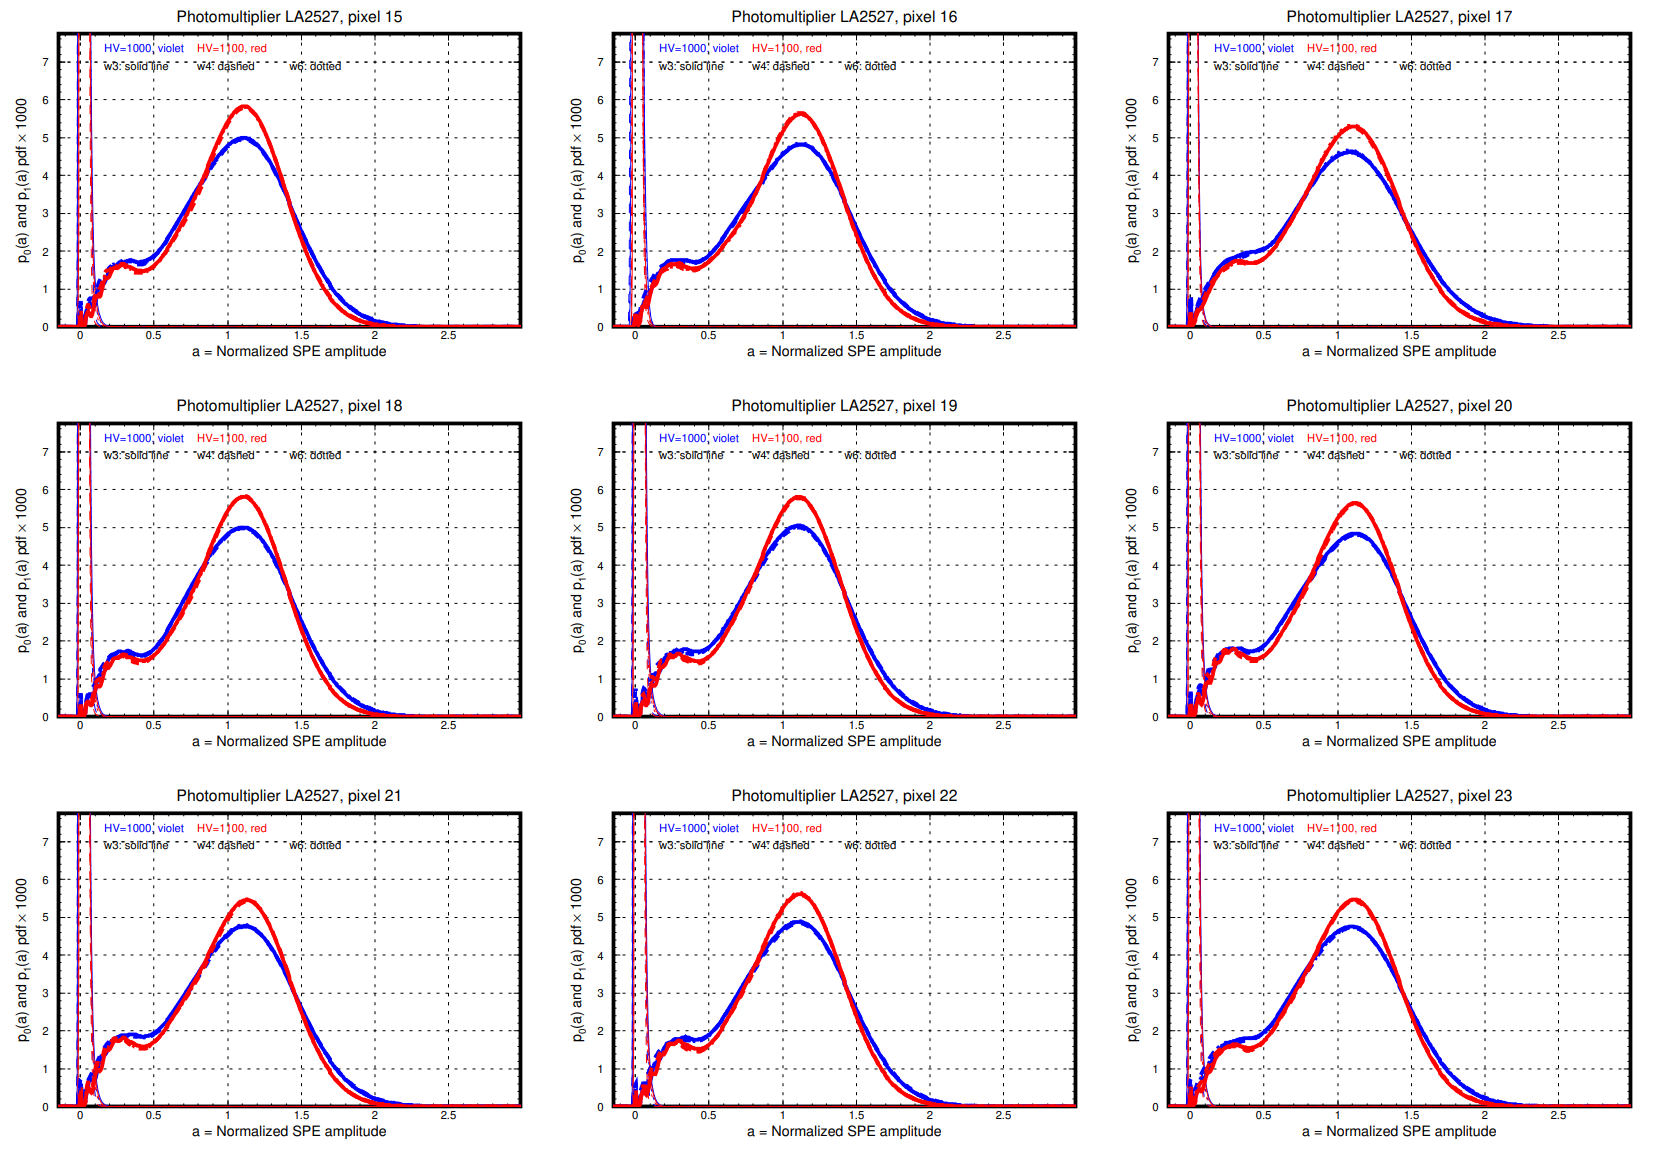
\includegraphics[width=1.0\textwidth,height=.7\textwidth]{figures/pavel_temp/LA2527_spectra_temp.png}
	\caption{Illustration of the ``MAPMT passport'' plots for one of the PMTs, LA2527 (H12700), continued. The standard six measurements included runs at three illumination settings (wheel positions 3, 4, and 6), each at two operating high voltages (1000~V, and 1100~V). Shown are the calculated SPE probability distribution functions $p_1(a)$, defined by the fit parameters resulting from the independent fitting procedures for each of the six settings. The blue color corresponds to the three sets at HV = 1000~V, and red - to the sets at HV = 1100~V. The parameters of the independent fits at three different illuminations result in very stable SPE shapes, essentially overlapping each other in the plots. The measurement functions $p_0(a)$ are shown as peaks around the pedestal at $a=0$ with the left sharp edge width corresponding to $\sigma$, and the right edge determined by the crosstalk.}
	\label{fig:LA2527_passport_spectra}
\end{figure*}

As a demonstration of the characterization procedure for the MAPMTs, Figs.~\ref{fig:CA7811}-\ref{fig:GA0516_4} show the measured signal amplitude probability distributions for one H8500 MAPMT pixel (CA7811, pixel 9) and one H12700 MAPMT pixel (GA0516, pixel 4) under various conditions, as well as their respective fit results. 
Figure ~\ref{fig:CA7811} and Fig.~\ref{fig:GA0516_1} illustrate the effect that the electronic crosstalk from neighboring pixels has on the measured SPE fit parameters. 
We collected two sets of data intended to reduce the contribution of crosstalk from neighboring pixels. In the first (as described in Section 4) we used a black sheet of paper to mask all pixels on a single MAPMT and punctured a 3~mm hole over the pixel of interest (see Fig.~\ref{fig:CA7811}a). 
However, with this setup, one cannot fully characterize the unmasked pixel, as there is some dependence of the measured signal on the location of the incident photon. 
To provide full coverage of a single pixel\textquotesingle s surface, another set of measurements was taken with a 6~mm x 6~mm square hole cut out over a single pixel. 
With this configuration, the full face of the pixel of interest was illuminated, while the neighboring pixels remained mostly covered by the black paper. 
However, there is still a non-negligible contribution from crosstalk with this configuration, due to imperfect alignment of the masks. 
This can be clearly seen in Fig.~\ref{fig:CA7811}b which shows the signal amplitude distribution with this 6~mm x 6~mm square hole cut out over pixel 9. 
One can see the contribution of the crosstalk appearing as a shoulder to the pedestal, albeit smaller than the crosstalk shoulder seen in Fig.~\ref{fig:CA7811}d where the full face of the MAPMT was illuminated. 

The resulting SPE fit parameters for Figs.~\ref{fig:CA7811}a-d indicate the inability of the model to fully describe the crosstalk in the H8500 MAPMTs. 
Most notably, in the data sets where the full-face of the MAPMT was illuminated (see Figs.~\ref{fig:CA7811}c-d) the $scale$ parameter changes by almost $7\%$ when the crosstalk is removed by the offline correlation analysis procedure compared to when it is kept in the data. 
Because the $scale$ parameter gives the average charge measured per photoelectron, it should be independent of the crosstalk. 
In contrast, we observe that the crosstalk in the H12700 MAPMTs can indeed be well described by the updated model, as is evident by comparing the fit parameters for Figs.~\ref{fig:GA0516_1}c-d. 
All parameters are consistent between the two fits, despite the fact that the crosstalk was removed by the offline analysis prior to performing the fit for Fig.~\ref{fig:GA0516_1}c. 
This result exemplifies the ability of the model to extract the SPE parameters from the measured signal amplitude distributions in a crosstalk-independent manner. 

The sample comparison between typical H8500 and H12700 MAPMTs as shown in Figs.~\ref{fig:CA7811} and \ref{fig:GA0516_1} generally confirms our decision to switch to H12700 as the MAPMT of choice for the RICH detector. In the previous study (Ref.~\cite{DEGTIARENKO20171}), using a different electronics front-end and data acquisition system, we observed that the values of the $\nu_{average}$ parameters were generally much smaller for H8500 than for the H12700, leading to a significant improvement of the expected efficiency of the H12700 MAPMTs to SPE events. In the previous study the amplitude resolution was not good enough to uncover the additional difference between the two models: the crosstalk spectra are significantly wider in the H8500, decreasing the expected SPE efficiency further, as compared to H12700. Wide crosstalk distributions in the H8500 overlap noticeably with the shapes of the model SPE functions and do not allow the model to isolate them, while for the H12700 MAPMTs the separation between the crosstalk and SPE distributions is reliable.  

The same sets of data were taken with the H12700 MAPMT high voltage set to 1100~V to compare with the results of Fig.~\ref{fig:GA0516_1} which were taken at 1000~V. 
The resulting amplitude probability distributions and fits are shown in Fig.~\ref{fig:GA0516_2}. 
As expected, both the $scale$ and $\nu_{average}$ parameters are larger when the high voltage is increased to 1100~V, while the parameters describing the crosstalk, $\beta/\mu$ and $\zeta/scale$, are fairly consistent. 
Furthermore, by comparing Fig.~\ref{fig:GA0516_2}c and Fig.~\ref{fig:GA0516_2}d, we observe the same desirable characteristic that the SPE fit parameters are consistent with or without the offline removal of the crosstalk events from the data even at a larger high voltage setting.


Finally, Fig.~\ref{fig:GA0516_3} and Fig.~\ref{fig:GA0516_4} show the signal amplitude probability distributions for the same pixel on MAPMT GA0516 at higher illumination intensities. 
Specifically, Fig.~\ref{fig:GA0516_3} shows the results with new light intensity for high voltage settings 1000~V and 1100~V, both with the full MAPMT face illuminated, and with the 6~mm x 6~mm square hole mask cutout applied. 
Comparing Fig.~\ref{fig:GA0516_3}c to Fig.~\ref{fig:GA0516_1}d (full-face illumination, 1000~V), the $\mu$ parameter is almost a factor of 10 larger for the data collected with the new light intensity, but the characteristic parameters for the SPE response are consistent. 
The same can be said by comparing to the signal amplitude probability distribution in Fig.~\ref{fig:GA0516_4}c, which was measured at even higher illumination.
Even at roughly 100 times the light intensity, the resulting $scale$ parameter is consistent to that measured at low light intensity. 

Figure~\ref{fig:LA2527_passport} shows an example of the ``passport'' plots obtained for a single MAPMT - in this case, an H12700 PMT labeled LA2527. 
Each plot shows different parameters extracted from the fits to the signal amplitude probability distributions vs. the pixel number, resulting in 64 data points per curve.
In all plots (excluding the top-right plot), the fit results are compared for the data taken with wheel positions 3, 4, and 6, and high voltages 1000~V and 1100~V (6 different configurations in total).
The wheel positions 3, 4 and 6 correspond to relative light intensities 1:5.63:1.68.
As expected the $scale$ and $\nu_{average}$ parameters are independent of the light intensity, but change with the applied high voltage. 
This is due to the increased amplification at each dynode at higher applied voltages.
The $\beta/\mu$ and $\zeta/scale$ parameters that describe the crosstalk from neighboring photoelectrons remain somewhat consistent between the different experimental configurations. 
However, the $\beta/\mu$ passport plot shows the dependence of the frequency of crosstalk on pixel location. For example, the first 8 and last 8 pixels all have significantly lower $\beta/\mu$ parameters. These pixels are along the edge of the MAPMT and therefore have (at least) one fewer neighboring pixel than those in the center of the MAPMT.
Consequently, the $\beta$ parameter for the amplitude probability distributions in these pixels is lower. 

The measurement of the absolute photon flux on each pixel was discussed in Section 5. 
The stability of the light flux was demonstrated by running the same PMT many time during the characterization.
The QE is obtained for each pixel by combining this measurement with the average number of photoelectrons measured per laser pulse, $\mu$, which is extracted separately for each pixel as a parameter of the fit to the signal amplitude probability distribution. The resulting QE distribution is shown in the top-right plot of Fig.~\ref{fig:LA2527_passport}. These results indicate that on average the QE for each pixel of the H12700 MAPMTs is about 21$\%$ for incident photons with wavelength 470~nm.

The lower-right plot illustrates the quality of the SPE fit by showing the standard $\chi^2/NDF$ values for every fit, calculated for all bins in the measured spectrum with amplitudes above threshold. The accumulated number of events in each measured spectrum was very high and it is hard to expect an ideal model description with $\chi^2/NDF = 1$. The statistical quality of the fit was reasonably good for all measured spectra.

One final remark from the plots included in Fig.~\ref{fig:LA2527_passport} is that the SPE efficiency shown in the lower-left plot is slightly larger at 1100~V than at 1000~V. The efficiency was defined as the percent of SPE events above the threshold, which, in turn, was defined as the amplitude at which the number of events in the SPE distribution below the threshold was equal to the number of events in the crosstalk spectrum above it. The higher voltage leads to increased separation between the SPE spectra and the pedestal, corresponding to larger values of $\nu_{average}$, and thus increasing the efficiency. 

Figure~\ref{fig:LA2527_passport_spectra} shows the extracted SPE functions for 9 pixels on the same MAPMT, again for all 6 configurations. The probability distributions are given as a function of the normalized charge amplitude, $a$. The functions extracted from the data measured at 1100~V are noticeably more narrow around the peak than the data collected at 1000~V, in agreement with the previously noticed differences between the values of $\nu_{average}$ and the efficiency at the different high voltages. The plots also illustrate the pedestal measurement functions around $a=0$, including the crosstalk contributions. The pedestal functions and the SPE functions, measured independently at three illumination settings, visibly overlap, and thus illustrate the stability of the fitting procedure and validate the applicability of the model in its function to objectively extract the MAPMT characteristics.


\iffalse
The performance of MAPMTs was evaluated under certain high voltages.
The single photoelectron spectrum and the pixel efficiency for H12700 MAPMTs were tested and analyzed at 1000v, 1050v, 1075v, and 1100v.
The measurements performed at the reference supply voltage of 1000 V were compared to the measurements at different HV values in order to study the behavior of the MAPMT response as a function of the supply voltage.
As expected, it was found that the H12700 MAPMTs perform the best in the single photoelectron spectrum efficiency at higher voltages, especially at 1100v.
We see a significantly improved separation of the first photoelectron peak from the pedestal at higher voltage supplies (see~Fig.~\ref{fig:SPEhv}).
When the average deficiencies of the tested MAPMTs were analyzed, it was found that the average efficiency for 1000v, 1050v, 1075v and 1100v were approximately 4.6\%, 4.9\%, 5.0\%, and 5.2\%, respectively.
Therefore, the increase in detection efficiency is found to be over 10\% at 1100 V in comparison to 1000 V supply.
This separation is the crucial point for a single photon counting detectors such as CLAS12 RICH, where the occupancy is at the level of one photon per pixel.



It was also found that as the gain of the MAPMT increased, the efficiency ratio of 1100v to 1000v decreased.
The ratio is shown on~Fig.~\ref{fig:effratio} as a function of MAPMT gain reported by Hamamatsu.
The high voltage supply improves the performance of MAPMT dynode system, decreasing the fraction of the single photoelectron events below the pedestal peak.
This indicates that lower gain MAPMTs have a greater difference in the efficiencies at 1100v and 1000v, while higher gain MAPMTs have a smaller difference between the two voltage efficiencies.
The improvement for lower gain MAPMTs is more significant than for higher gain MAPMTs, because the high gain MAPMT has good separation of signal from pedestal even at the reference 1000 V.
Therefore, the low gain MAPMT benefit greatly from higher supply voltage.
The collected data are used to determine what high voltage the MAPMTs should be ran at to acquire the best results when the RICH detector is completed.


The parameters from Pavel's PMT response function are shown on the Fig.~\ref{fig:mu} and \ref{fig:characteristicPars} and correspond to the emission of the photoelectron ($\mu$), its collection and multiplication on the first dynode ($scale$ and $\nu$).
We have omitted other parameters that take into account the resolution effects of readout system or correspond to the cascade multiplication of the secondary electrons as they are out of scope focus of our analysis.
Given our requirements for single photoelectron signal sensitivity MAPMTs of our choice should be able to detect with high probability single photon that reaches photocathode.
In order to achieve this goal MAPMT should have high quantum efficiency of the photocathode as well as high collection efficiency of produced photoelectron combined with substantial signal multiplication to achieve good resolution of SPE peak.
These characteristics were studied in bulk for all 27520 channels (430x64) during the different light conditions and for different supplied HV values.


Fig.~\ref{fig:mu} shows the distribution of parameter $\mu$ which correspond to the average number of the photoelectrons produced during the measurements.
This parameters represents the convolution of the MAPMT photocathode quantum efficiency and laser setup light intensity.
Both characteristics should not depend on HV supply values and it is demonstrated on this figure by comparison of $\mu$ values extracted for the measurements at 1000 V and 1100 V.
However one can change the parameter by varying the laser light intensity which is evident from the left shift of $\mu$ values for lower light intensity measurements.

The other two free parameters are plotted on Fig.~\ref{fig:characteristicPars}.
They correspond to the average number of second-stage electrons produced on the first dynode by photoelectron (see~Fig.~\ref{fig:nu} and average signal amplitude for single photoelectron spectrum (see Fig.~{fig:scale}).
Both parameters characterize mainly the amplifying subsystem of MAPMT and therefore should depend on supplied HV.
The measurements at 1000 V and 1100 V confirm that amplification is improved at higher values of applied high voltage.
Traditionally the second parameter (gain) is often used to describe the amplification abilities of photomultipliers and often used in calibration and reconstruction procedures.
And it was shown that the extracted gains do not depend on the light conditions with a high degree of accuracy.
\fi
